% 10ish pages, about 8 in text, about 2 in figures
% Results had 18 pages, 50/50 ish split
% probably some 20ish pages here
\chapter{Evaluation}

% Stuff that goes here:
% Faas-sim: what is it, how does it work, what are its models, how does it deal with containers/kubernetes/openfaas/etc. What is simulated, what isn't? How are network flows simulated?
% Request pattern stuff.
% what types devices are there
% what functions are there, how do they perform on each device?
% image sizes, pulls, request payload sizes, all that stuff
% topologies: What are there and how are they built? real measurements from papers, etc. etc.
% -> city level, both old and modern, visualizations, etc.

% practical: how did we eval traefik
% real cluster, galileo (briefly), what devices are there? Auto-responder type app, payload size, response time, etc.

% Experiments:
% 1) Prelims
% 2) traefik resource eval
% 3) more realistic topo
% 4) load balancer count tests
% 5) LB hyperparameter tests
% 6) the osmotic stuffs?

This chapter describes the experiments we conduct as well as their results.
First, we described the initial evaluation we performed which significantly informed our exact approach.
It provides first insights into the performance improvement one can expect, and also helps uncover potentially unexpected system behaviour.
After this initial set of experiments we continue our evaluation with the implementation and parameter configuration of the load balancers.
From there we continue with experiments related to the effect and cost load balancers have.
As we described, our serverless function simulator uses real-world values whenever possible to inform its simulation.
To this end we test the resources used by a single load balancer instance under various conditions on different kinds of hardware.
Because the overall resource cost load balancers incur is a function of the resource consumption of each instance and the number of instances deployed, we next evaluate load balancer scale.
Lastly we evaluate our osmotic scaling and scheduling approach.
We start this evaluation by testing how our osmotic scaling behaves under more realistic system conditions, as well as how it affects the serverless system.
Next, we test the effect of different pressure thresholds on system performance.
Combined with previous experiments this informs how scaling parameters result in different levels of performance and load balancer resource consumption.
The last experiment conducted tests how our osmotic approach handles dynamically changing system conditions, exploring how the scaler and scheduler behave when requests change their origin within the system over time.

\section{Initial Assessment}
% good 3-4 pages

\section{Load Balancer Implementation and Parametrization}
Next, we explore the effect the load balancer implementation and parametrization have.
Because the edge computing environment features different conditions than the cloud, we evaluate whether or not different implementations of weighted round robin affect the system differently.
In addition we evaluate the parameter configuration for our load balancing approach, testing if there are certain configurations that perform better than others and trying to see if there are patterns in the parameters' influence on performance.
\section{Least Response Time Load Balancing Implementation}
% 2 pages
\section{Load Balancer Parametrization}
% with graphics 2 pages -> with graphics got 5-6 pages.
With this range of experiments we set out to better understand the effects different parameters have on a load balancers performance.
We then continue to use this information to make an informed decision for the load balancer parameters in subsequent experiments.

Specifically, we want to understand the relationship between the following load balancer parameters:
\begin{enumerate}
    \item \textbf{Scaling Factor:} the factor which determines how linearly observed node performance is mapped to weights
    \item \textbf{Weight Range:} the size of the weight range the load balancer can use
    \item \textbf{Current Weight Reset:} whether or not it makes sense to reset the current weights of the load balancers when the weights are changed
\end{enumerate}

\subsection{Setup}

Since previous experiments have shown that the impact parameter changes can have are at times hard to predict, we decided to perform this evaluation using a grid-search, meaning that we rely on trying a large number of permutations to find patterns in their behaviour.
To test these settings we do not rely on the full FaaS-Sim environment, but rather perform isolated tests with a single load balancer and less sophisticated function and network simulations.

Since we are trying to evaluate how well load balancers choose upstreams, the upstreams are the comparatively most accurately simulated component.
The performance model of our simulated upstreams is closely informed by our notion of a node's performance level and capacity, which we outlined in our load balancing approach.
Thus, each simulated upstream has a set level of performance, which determines how long it takes for a request to be processed.
Since our aim is to keep this simulation simple, we consider the response time determined by the upstream to represent both the network and the \gls{fet} that would be observed in a real serverless system.
Each upstream samples its response times from a set of two lognormal distribution, one of which represents the \gls{fet}, while the other represents the network time.
To simulate the effect of high load, each upstream also has a set capacity, measured in requests per second.
If an upstream receives more requests per second than is has capacity for, \glspl{fet} start to degrade linearly, meaning that response times get longer in proportion to how overloaded the upstream is.

To represent different system conditions we introduce \textit{performance spread} as an input variable to these experiments that determines the how heterogeneous the performance of the simulated upstreams is.
The assumed system scenario is closely aligned with the one of our initial evaluation.
Relative to the load balancer a node can fall into one of four location categories, which determine the network distance from the load balancer: \textit{local}, \textit{city}, \textit{nation}, and \textit{global}.
Like it would  be in a real scenario, the probabilities of nodes falling into each of the categories gets progressively higher, meaning that a very low number of nodes will be local, while the majority will be \textit{global} and thus rather far away form a network perspective.
Apart from their location, nodes can fall into three performance categories, which are \textit{small}, \textit{medium}, and \textit{large}.
This performance category determines both the typical \gls{fet} of that node and its capacity.
Small and medium nodes are more likely to be located close to the load balancer, while large nodes are likely to be farther away in the network.
This is done to represent a typical edge computing scenario where relatively weaker compute is available locally, with a large amount available farther away, e.g. in the cloud.
The performance spread then determines how big the differences between the different categories nodes can fall into are.
A performance spread of 15 for example would correspond to as scenario where \glspl{fet} range from 10ms to 150ms, capacities from 5\gls{rps} to 100\gls{rps}, and network times from 5ms to 250ms.
A higher performance spread would indicate higher performance differences, while a lower one would indicate lower differences, with a performance spread of 1 indicating complete homogeneity.


To make an informed decision on load balancer parametrization we performed three experiments.
\subsubsection{Scaling Factor and Performance Spread}
In this evaluation we examine the effect the scaling factor has on performance in a variety of different scenarios.
To this end we tested scaling factors from 0,1 to 10.
Scenarios included performance spreads from 1 to 46, and all scenarios were repeated three times with request loads of 50\gls{rps}, 250\gls{rps}, and 1000\gls{rps}.
The weight range upstreams were mapped onto in this experiment is [1;10].
The experiment covers a simulated time frame of 1000 seconds.

\begin{figure}
    \centering
    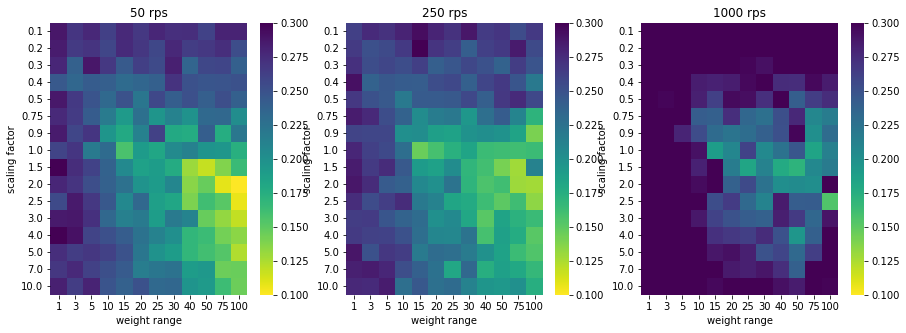
\includegraphics[width=14cm]{graphics/graphs/lb_hyper_scaling_vs_performance_spread.png}
    \caption{Mean response time over various levels of performance spread and scaling factors}
    \label{fig:lb_hyper_scaling_perfspread}
\end{figure}

The results of this experiment can be seen in Figure \ref{fig:lb_hyper_scaling_perfspread}.
Aside from showing lower performance for higher performance spreads, which is entirely to be expected since a larger performance spread means nodes are farther away and have higher \glspl{fet}, there are no significant differences between the scaling factors.

\subsubsection{Scaling Factor and Weight Range}
Analogously, we also evaluated the relationship between the scaling factor and weight range using a grid-search type experiment.
We once again tested scaling factors in the range [0,1;10] with request loads of 50\gls{rps}, 250\gls{rps}, and 1000\gls{rps}.
For the weight range the minimum weight was always set to 1, and the max weight between 1 and 100.
The performance spread was fixed over all experiments at 15, and the simulation is again run for 1000 seconds.

\begin{figure}
    \centering
    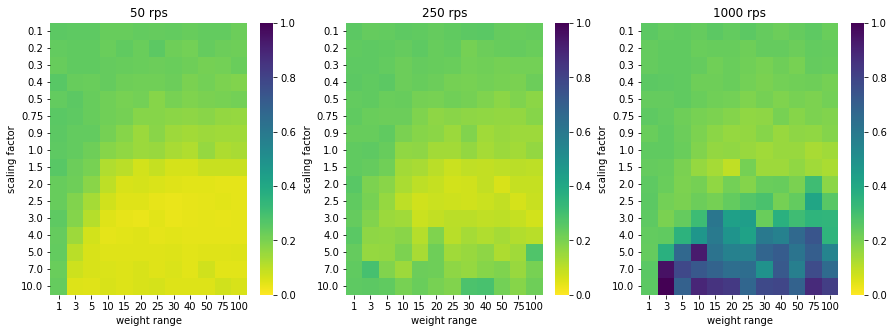
\includegraphics[width=14cm]{graphics/graphs/lb_hyper_scaling_vs_weight_range.png}
    \caption{Mean response time over different weight ranges and scaling factors}
    \label{fig:lb_hyper_weightrange_scaling}
\end{figure}

The results of this evaluation can be seen in Figure \ref{fig:lb_hyper_weightrange_scaling}.
Results show a clear trend towards higher weight ranges and scaling factors that are close to or slightly above 1, which would correspond to linear scaling.
We can also observe that higher request loads lead to worse performance on average, as one would expect, and also seem to shrink the set of configurations that provide good performance.

\subsubsection{Resetting Weights on Updates and Weight Update Intervals}
Our implementation of weighted round robin described earlier has a set of two weights for each upstream: the weight, and the current weight.
Once the weight of an upstream changes, we can choose to also reset the current weight or leave it as is.
Since intuitively there was no clear answer as to which choice is better, and the testing infrastructure around this was already in place, we chose to perform an experiment to measure the impact of this choice.
Apart from whether or not weights should be reset on updates, one also needs to decide at which interval weight updates should occur.
To evaluate this choice we performed these experiments using a variety of different update intervals.
Since we expected that resetting weights will have an outsized effect for scenarios with a low request rate, we performed experiments over a wider range of request loads than before, and also tested over different weight ranges.
Request load ranges from 2\gls{rps} to 1000\gls{rps}, weight update frequency from 5 seconds to 200 seconds, and maximum weight once again from 1 to 100.
Lastly, all experiments simulated a timeframe of 1000 seconds.

\begin{figure}
    \centering
    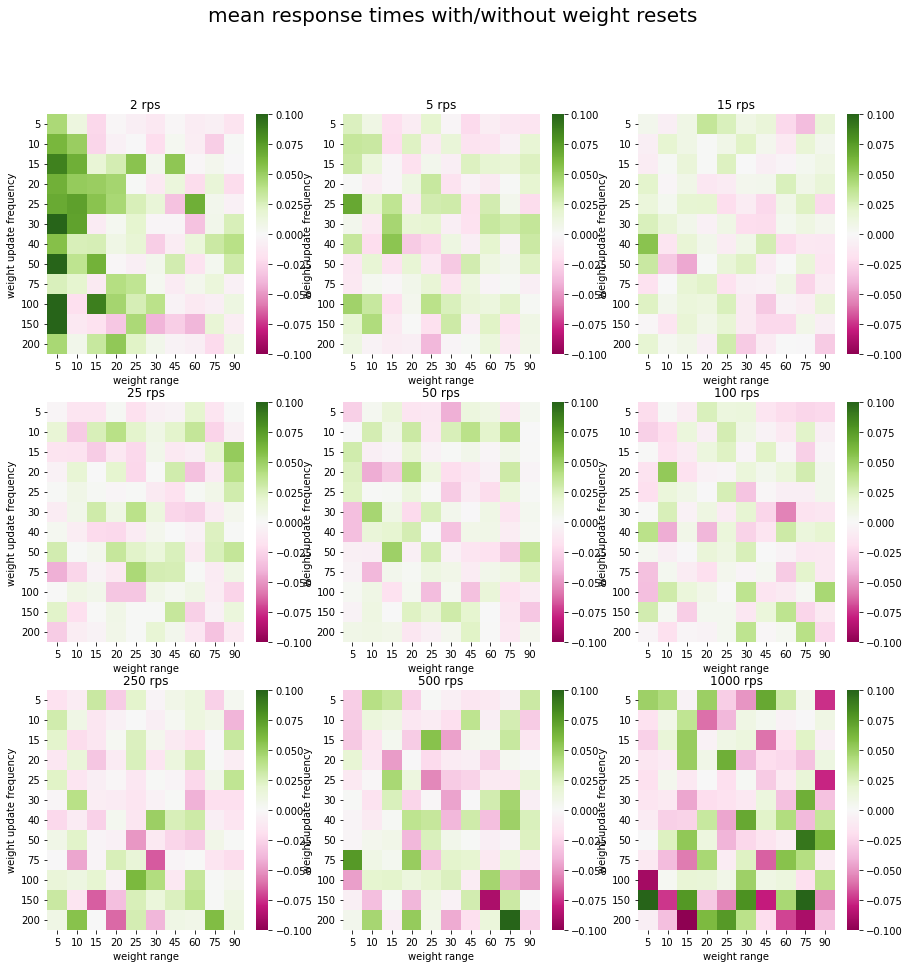
\includegraphics[width=14cm]{graphics/graphs/lb_hyper_weight_reset_delta.png}
    \caption{Difference between resetting and not resetting weights on update. Positive values indicate not resetting performs better, while negative values indicate the opposite.}
    \label{fig:lb_hyper_reset_delta}
\end{figure}

\begin{figure}
    \centering
    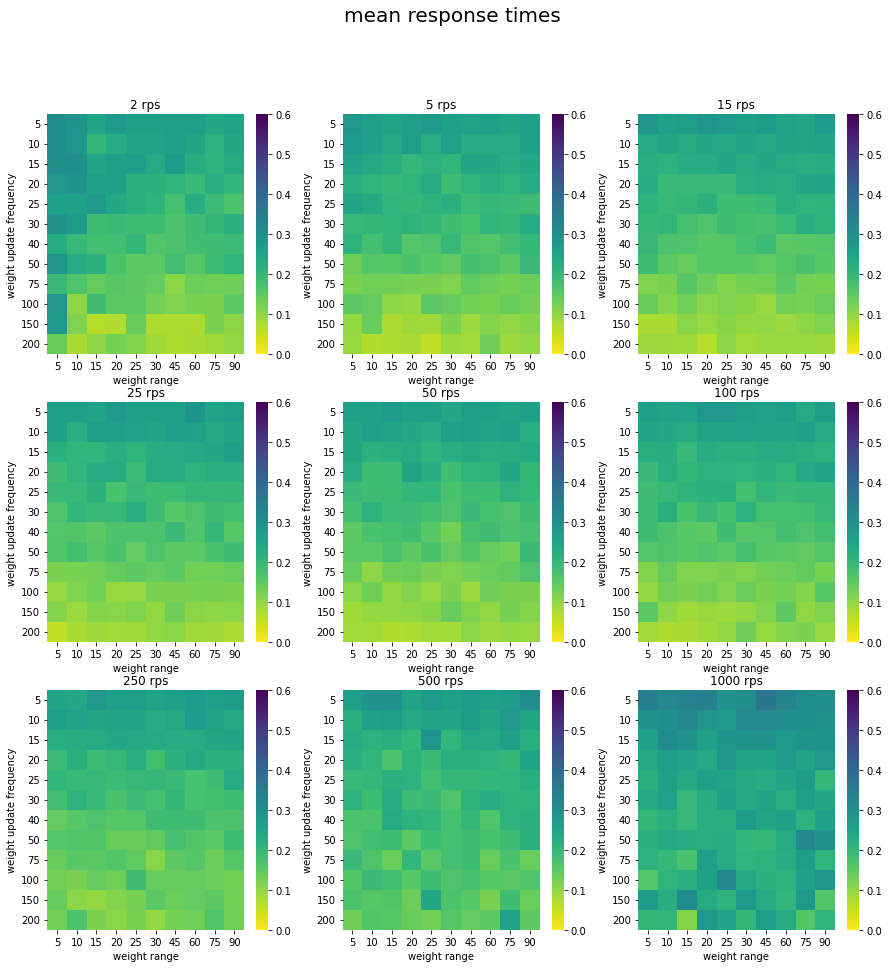
\includegraphics[width=14cm]{graphics/graphs/lb_hyper_mean_with_reset.png}
    \caption{Mean response times over different weight ranges and weight update times. Current weights are reset on update.}
    \label{fig:lb_hyper_reset_mean}
\end{figure}

\begin{figure}
    \centering
    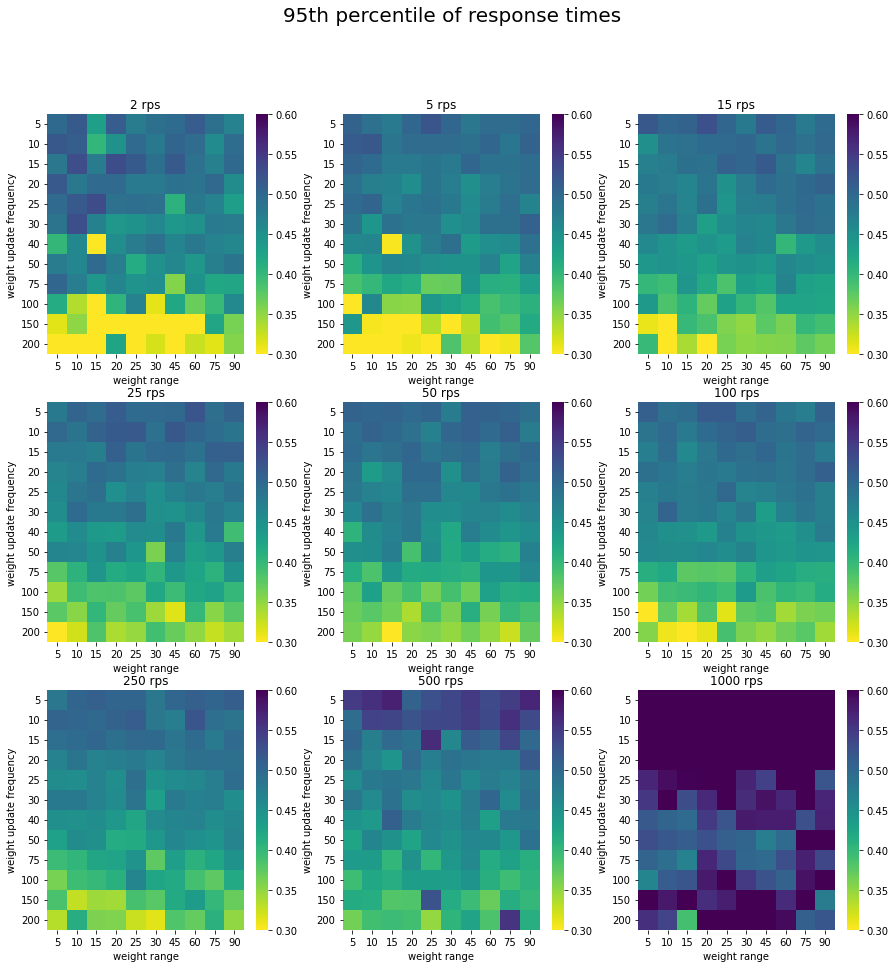
\includegraphics[width=14cm]{graphics/graphs/lb_hyper_95th_percentile_with_reset.png}
    \caption{95th percentile of response times over different weight ranges and update times. Current weights are reset on update.}
    \label{fig:lb_hyper_reset_q95}
\end{figure}

Figure \ref{fig:lb_hyper_reset_delta} shows the difference between the mean values of resetting or not resetting current weights.
In the results there is no clear indication resetting or not resetting is clearly superior.
There is a slight trend for not resetting performing better with low request rates, and resetting leading to better results in very high \gls{rps} scenarios.

Figure \ref{fig:lb_hyper_reset_mean} shows a trend towards longer intervals for weight updates performing better, irrespective of the weight range.
Figure \ref{fig:lb_hyper_reset_q95}, which shows the 95th percentile of the same data generally indicates the same tendency, although not for all request levels.
While at low request rates long update intervals perform better, they perform worse than shorter update intervals for high request rates.
Lastly we advise that care should be taken when comparing these visualizations, as the scale sometimes differs.
This is always indicated on the side of the visualization, and was necessary to better show relative differences within the same experiment run.


% Notes for discussion:
% QoS issue where one setting might be good under certain conditions, but bad under others e.g. 95th percentile type stuff
% extremes seem not to do so well for the most part
% behavious is to a large degree as expected: for low RPS super steep scaling works fine, but it becomes less good once capacity of the best nodes is reached
% No super clear point for or against weight resetting, once again depends on situation -> this points to a further investigation of the role of node discovery.
% to a degree weight resets perform a bit as expected in that low rps strongly prefer not resetting, and high rps preferring resets
% explanation why is quite intuitive, especially w.r.t. 

\section{Resource Usage and Load Balancer Scale}
After load balancer implementation and parametrization have been evaluated, we now move on to load balancer resource usage and scale.
The initial evaluation already shows that having distributed load balancers improves system performance.
With larger numbers of load balancers also come increased resource costs, however.
To find out the exact resource costs we measure the system resource usage of our load balancing approach on different physical hardware.
The second factor influencing the overall cost of distributed load balancers is the number of load balancers deployed.
Intuitively a greater number of load balancers will result in better overall performance, as load balancers will then have a better chance at being close to clients and function replicas.
In the second evaluation we explore the relationship between load balancer scale and system performance.
Together these two evaluations give us the insight needed to make an informed trade-off between total resource consumption and system performance.
\section{Load Balancer Resource Usage}
% 2 pages
\subsection{Performance Impact of Load Balancer Scale}
% 1 page
With this experiment we evaluate the effect different load balancer scales have on the system.
As we already described the quality and thus resulting end user performance of load balancer decisions only stabilizes after a while, since the load balancer first has to evaluate the available upstreams by sending requests to them.
Because of this, having larger numbers of load balancers present in the system might lead to delayed convergence, and thus suboptimal performance.
Having too few load balancers, on the other hand, might lead to lost performance through overly long routes.

To find out how different scales affect the overall system, we test the system performance with fixed percentages of nodes hosting load balancers.
We test a ranges between 5\% and 100\% of nodes hosting load balancers, which in our scenarios across three cities and 400 nodes means between 20 and 400 load balancer instances.
Scheduling load balancer replicas in these scenarios is still left to the Kubernetes scheduler, which means that the location of the node in the topology is not taken into account.

When testing ratios where less than 5\% of nodes hosted load balancers, we ran into frequent occurrences of the simulation not terminating within a feasible time window.
Upon investigation it turned out that if a load balancer was the only one in the city, or otherwise handled a lot of traffic, but happened to be placed onto a node with very limited bandwidth, the network simulation would take an exceedingly long time, because the bandwidth bottleneck resulted in each request only receiving a minuscule amount of bandwidth.
Requests that did go through took so long, that in real-life it would be considered a failed request by timeout.
We take this as an indication of the inherent problematic of current replica scheduling methods in edge computing, and that the usage of current techniques would simply require an outsized number of load balancers to mitigate the risk of such dysfunctional configurations.

The topologies tested are structurally similar to those of the initial evaluation.
Our two testing scenarios are three cities distributed across the United States, and three cities distributed across the globe.
The cities are identical to the ones from the initial evaluation, and feature identical network latencies between them.
The difference between these and the ones of the initial evaluation is that these feature a different internal topology, which is more closely related to edge intelligence\cite{rauschEdgeIntelligenceConvergence2019} and edge computing in general.
The cities in this evaluation have their compute capabilities, i.e. the cluster nodes, either in the city's local cloud data center, on a smart pole, or next to a cellular base station.
Clients are attached either to smart poles or directly to cellular base stations.
Cellular base stations themselves have a high-speed, high-bandwidth uplink to the wider network and feature a lower bandwidth and higher latency wireless connection to the clients.
These wireless properties depend on whether the cellular tower is LTE or 5G based, as both types are present in our scenario and their network properties are based on real world data\cite{braudMulticarrierMeasurementStudy2019}.
Not all cellular towers have directly attached compute capabilities.
In addition, one of the three cities does not feature a data center.

We simulate the cluster over the course of 2000 seconds, once with 25 \gls{rps}, once with 75\gls{rps}.

\begin{table}[]
\begin{tabular}{lrrrr}
\hline
                                                                             & \multicolumn{4}{c}{mean}                                                                                                                                                                                                                                              \\
\textbf{\begin{tabular}[c]{@{}l@{}}Nodes with\\ Load Balancers\end{tabular}} & \textbf{\begin{tabular}[c]{@{}r@{}}Global\\ 75rps\end{tabular}} & \textbf{\begin{tabular}[c]{@{}r@{}}Global\\ 25rps\end{tabular}} & \textbf{\begin{tabular}[c]{@{}r@{}}Nation\\ 75rps\end{tabular}} & \textbf{\begin{tabular}[c]{@{}r@{}}Nation\\ 25rps\end{tabular}} \\ \hline
\textbf{5\%}                                                                 & 210ms                                                           & 132ms                                                           & 220ms                                                           & 141ms                                                           \\
\textbf{10\%}                                                                & 149ms                                                           & 128ms                                                           & 158ms                                                           & 133ms                                                           \\
\textbf{20\%}                                                                & 134ms                                                           & 127ms                                                           & 147ms                                                           & 128ms                                                           \\
\textbf{30\%}                                                                & 132ms                                                           & 124ms                                                           & 141ms                                                           & 127ms                                                           \\
\textbf{40\%}                                                                & 130ms                                                           & 126ms                                                           & 135ms                                                           & 126ms                                                           \\
\textbf{50\%}                                                                & 128ms                                                           & 125ms                                                           & 134ms                                                           & 125ms                                                           \\
\textbf{60\%}                                                                & 129ms                                                           & 126ms                                                           & 133ms                                                           & 126ms                                                           \\
\textbf{70\%}                                                                & 129ms                                                           & 125ms                                                           & 128ms                                                           & 126ms                                                           \\
\textbf{80\%}                                                                & 128ms                                                           & 128ms                                                           & 131ms                                                           & 125ms                                                           \\
\textbf{90\%}                                                                & 129ms                                                           & 125ms                                                           & 129ms                                                           & 125ms                                                           \\
\textbf{100\%}                                                               & 127ms                                                           & 125ms                                                           & 129ms                                                           & 126ms                                                           \\ \hline
\end{tabular}
\caption{Mean \gls{trt} values of different load balancer scales, once they have converged to a stable value}
\label{tab:lb_scaling_converged_trt}
\end{table}

\begin{figure}
    \centering
    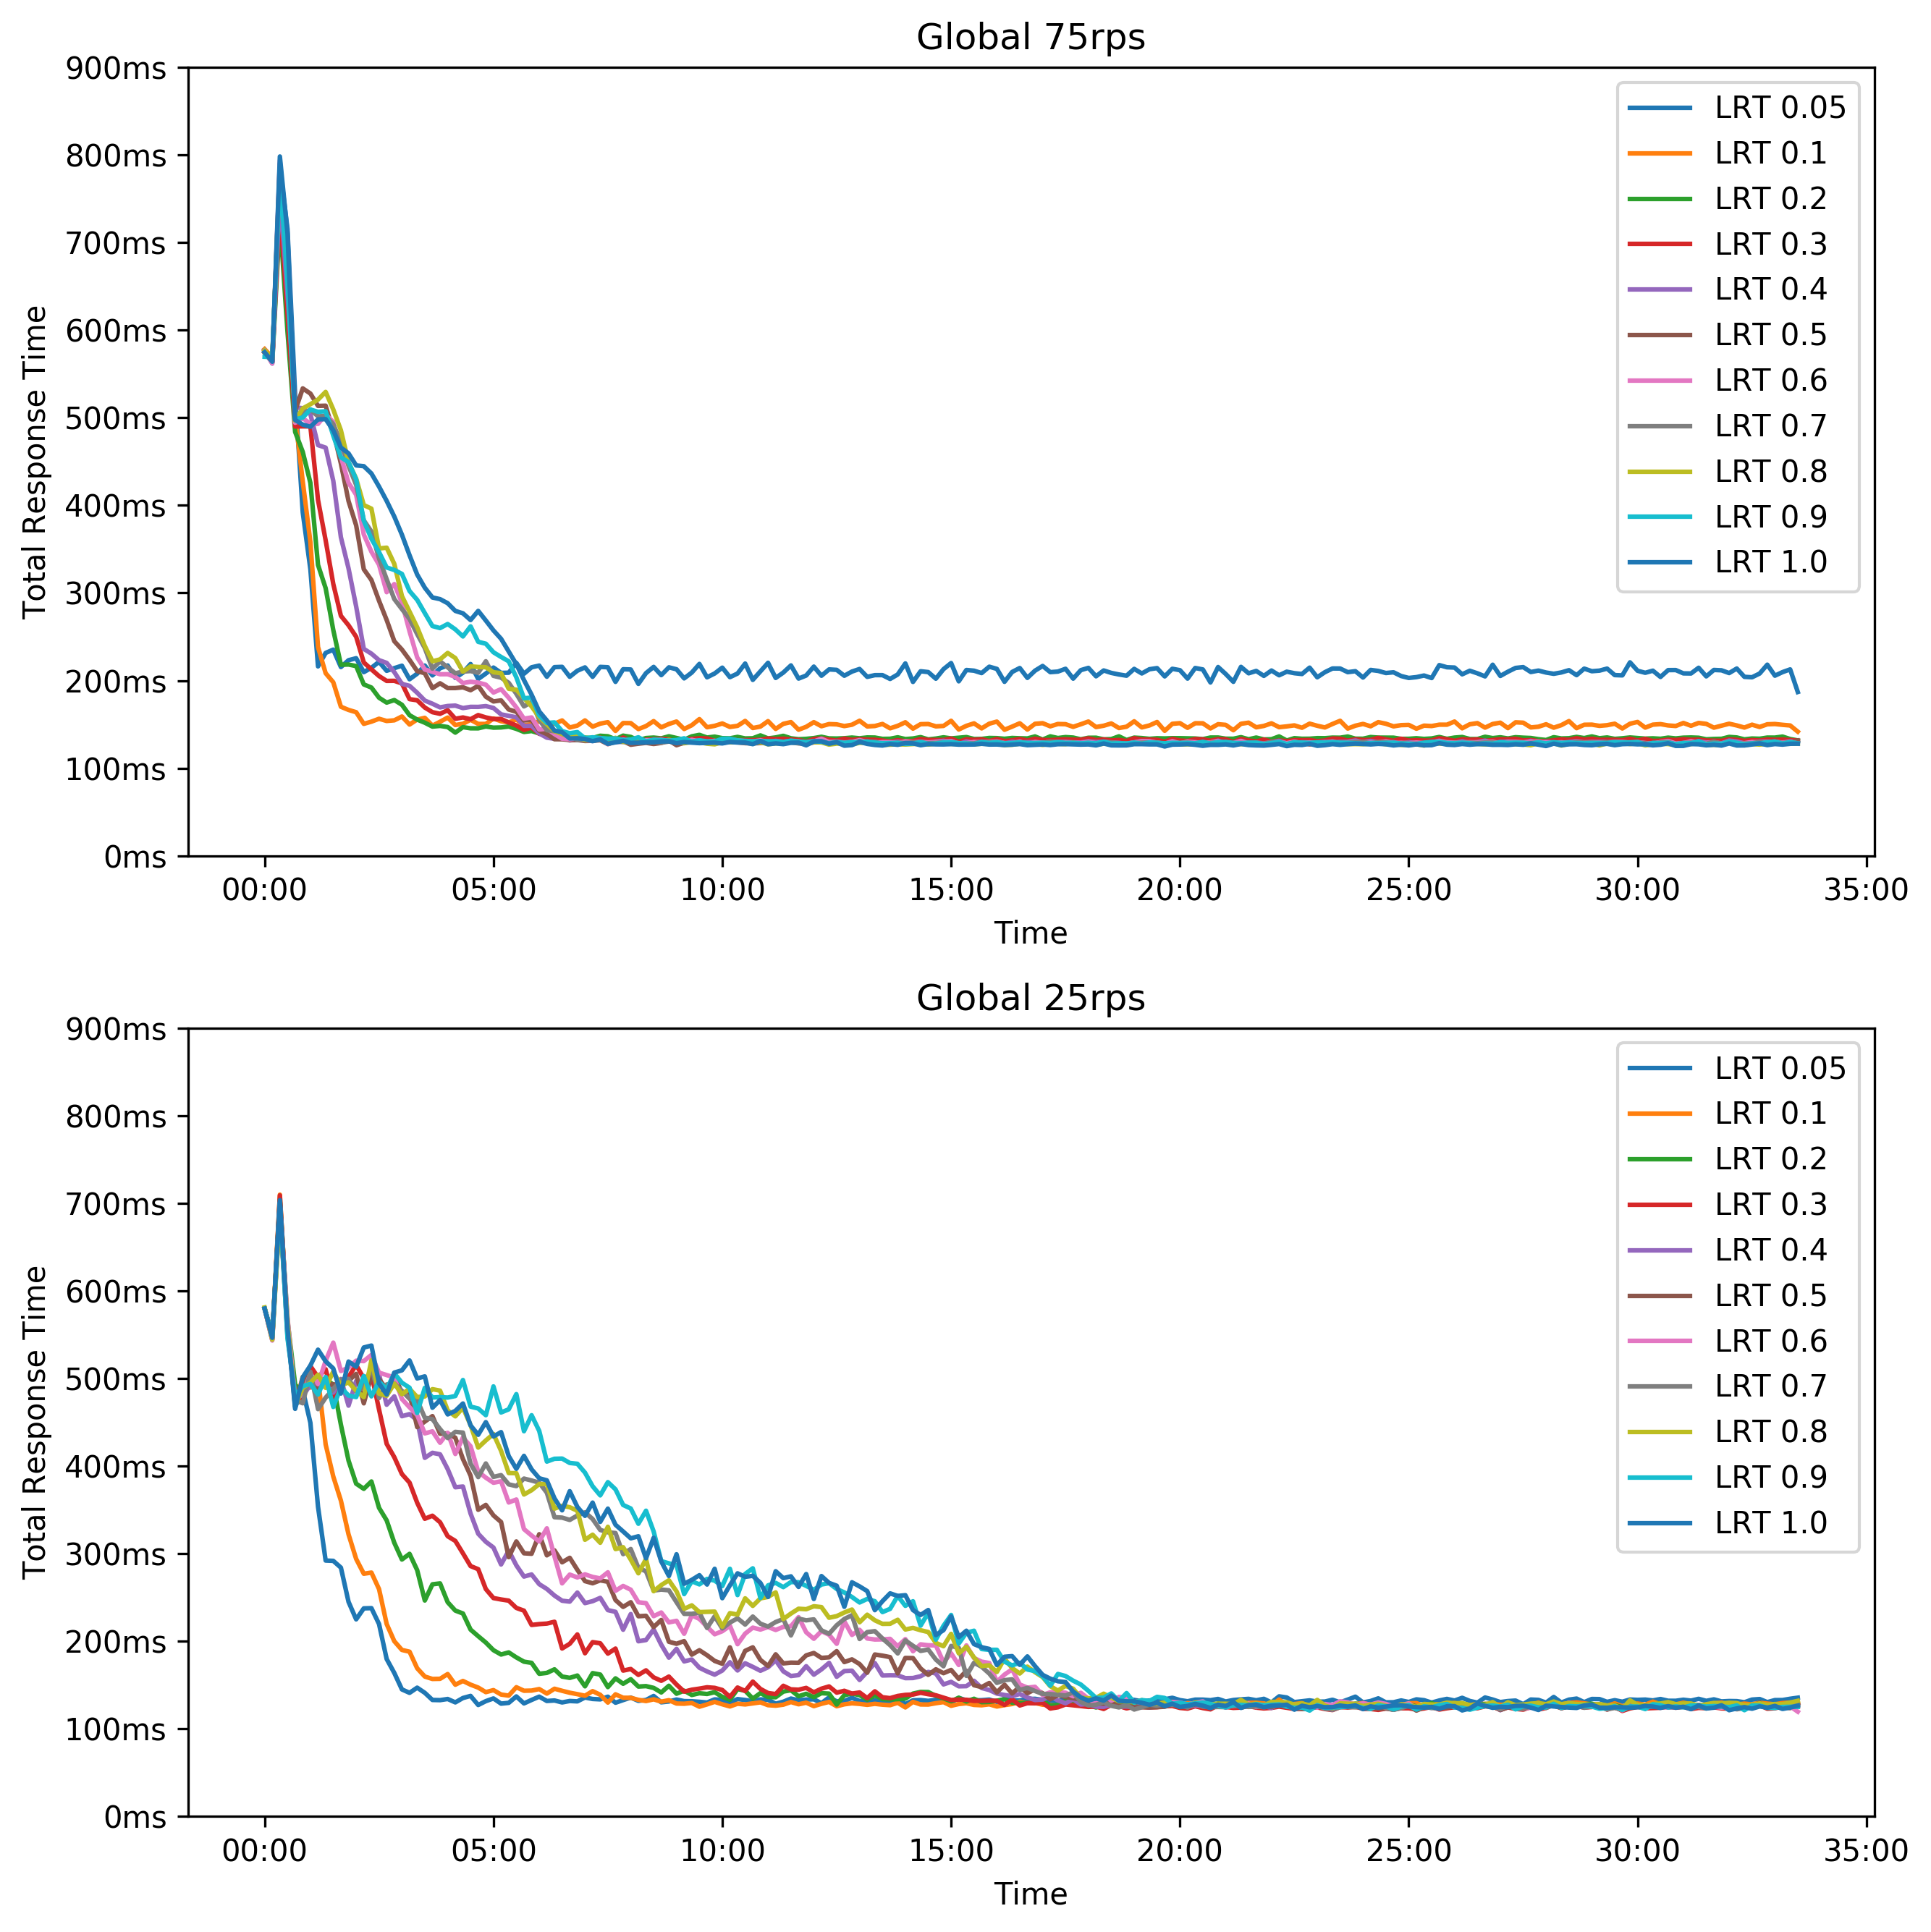
\includegraphics[width=\linewidth]{graphics/graphs/global_lb_scale_corrected.png}
    \caption{\glspl{trt} of different load balancer scales in the global scenario. For legibility a 10 second moving average is applied.}
    \label{fig:lb_scale_global}
\end{figure}

\begin{figure}
    \centering
    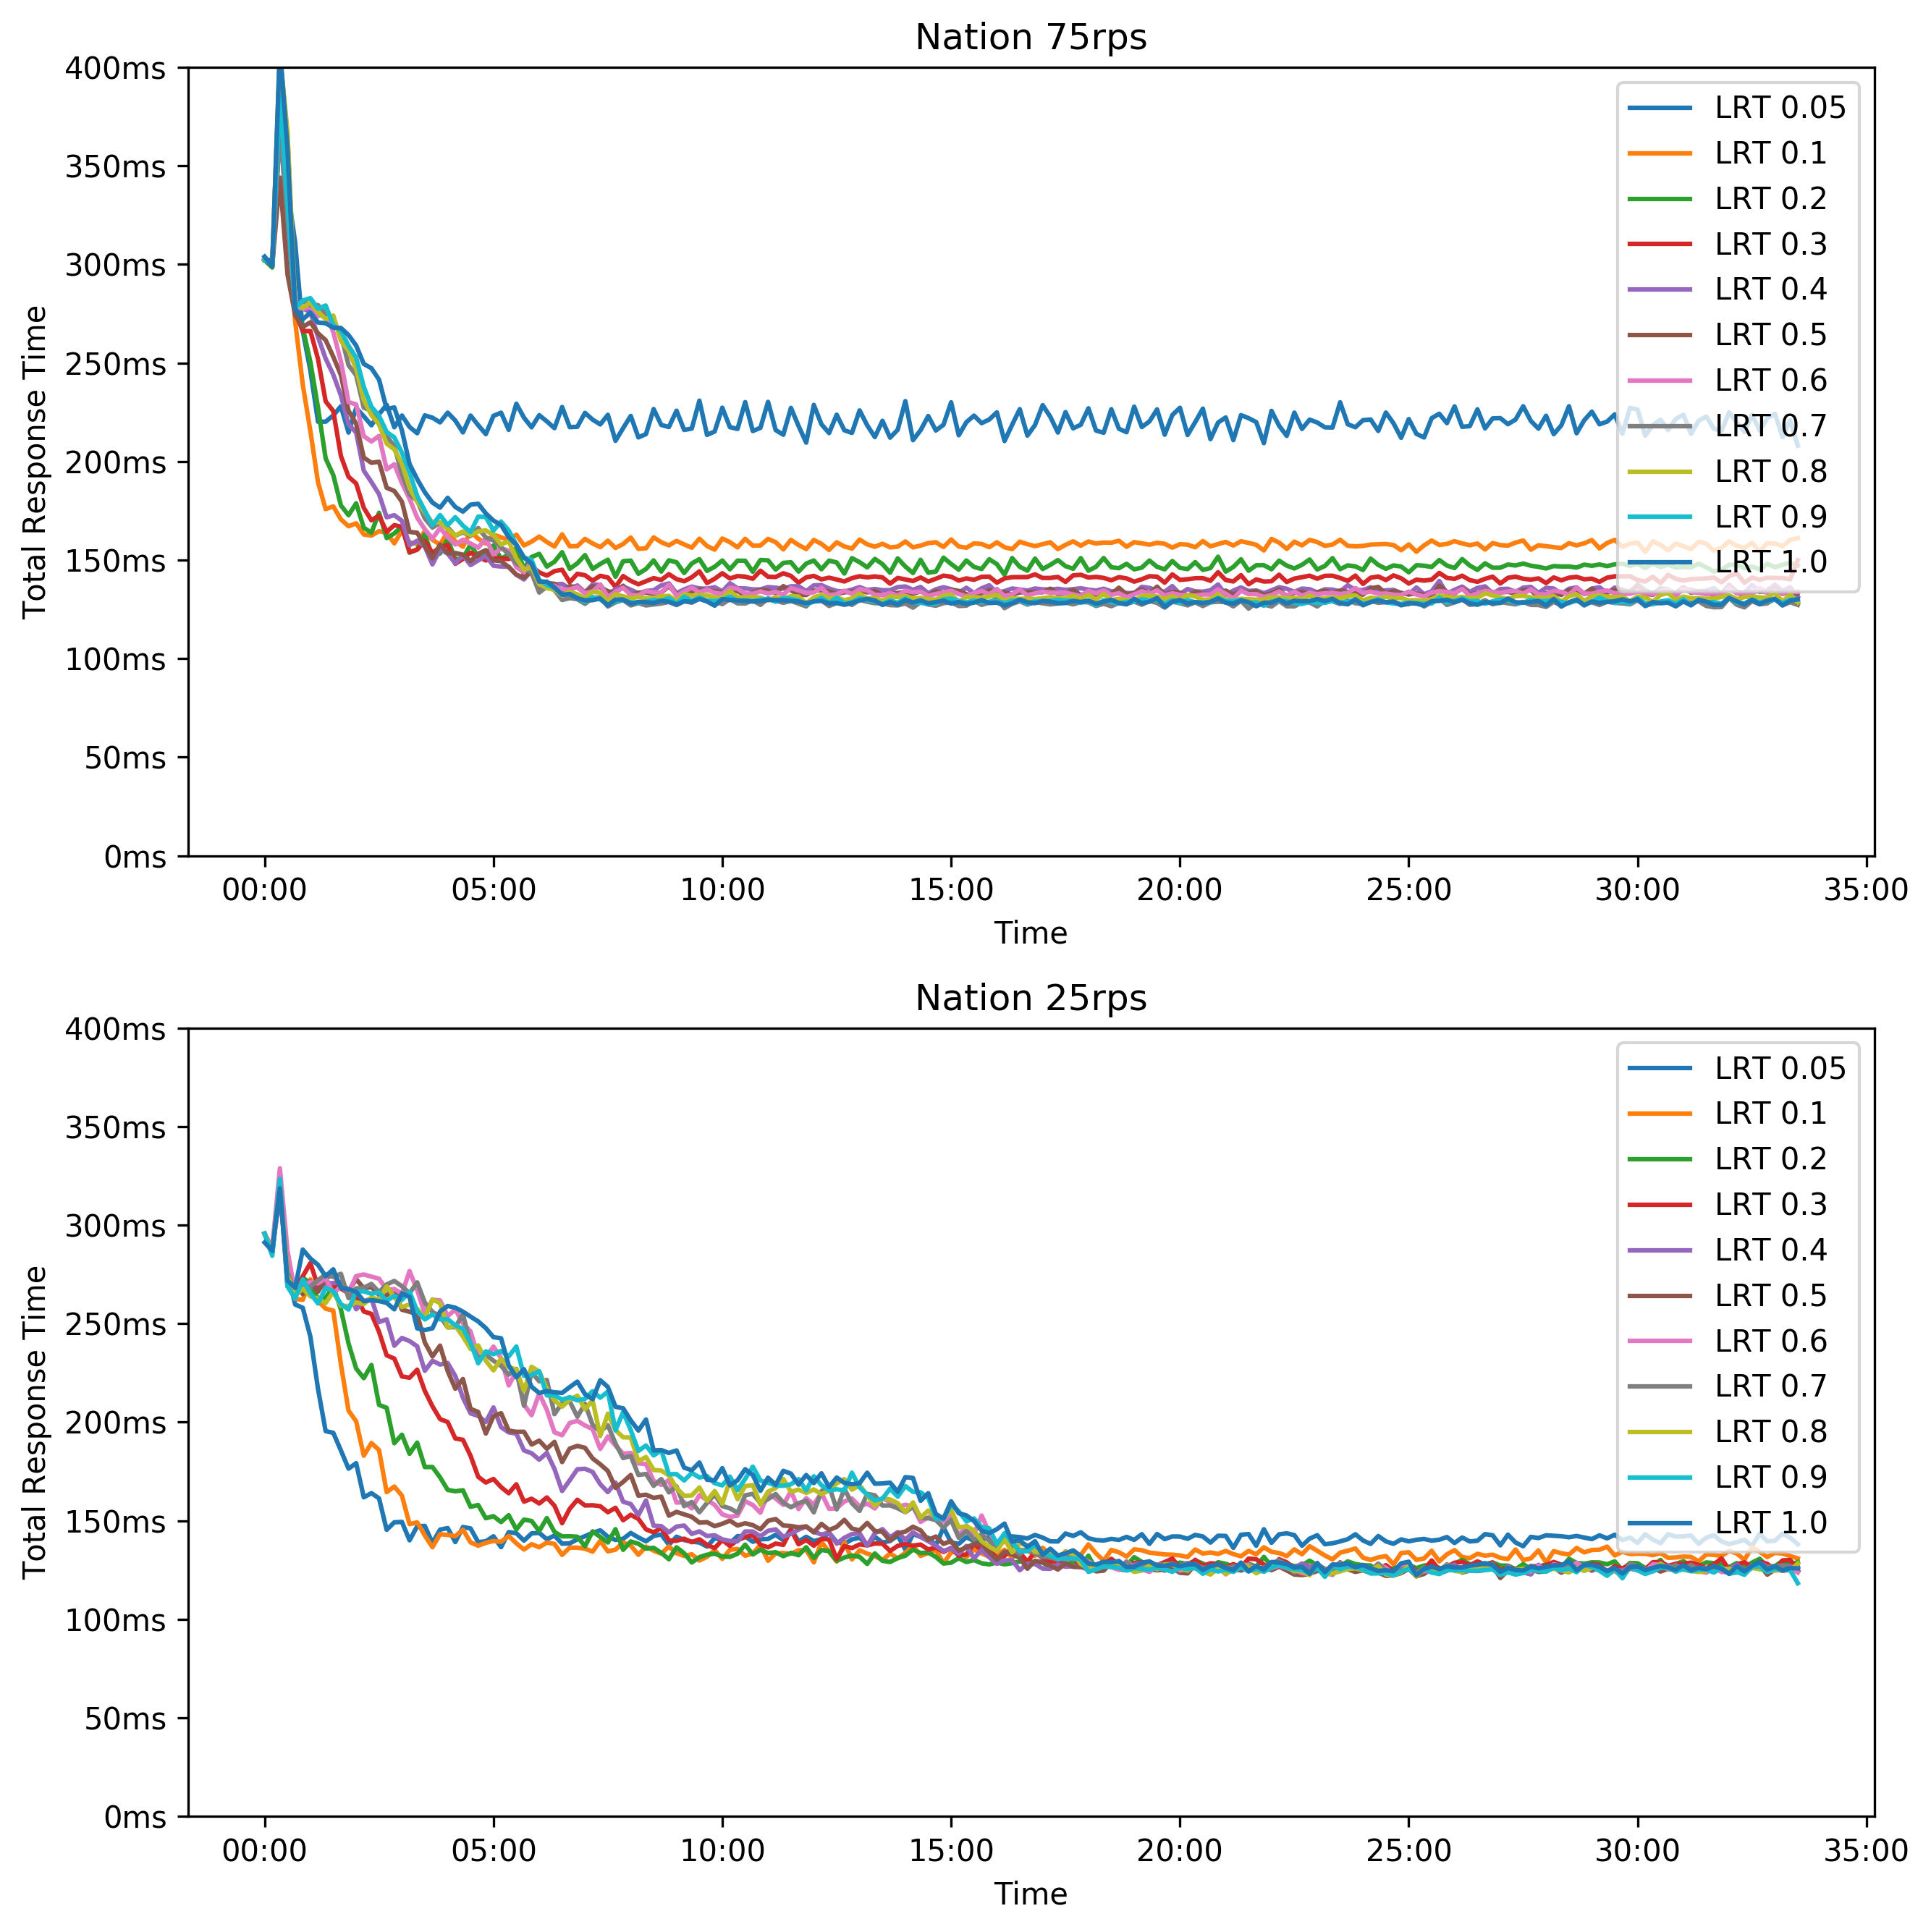
\includegraphics[width=\linewidth]{graphics/graphs/nation_lb_scale_corrected.png}
    \caption{\glspl{trt} of different load balancer scales in the nation scenario. For legibility a 10 second moving average is applied.}
    \label{fig:lb_scale_nation}
\end{figure}

Our results show consistent patterns across both topologies, but differ across the request rate.
While in scenarios with a request rate of 75 \gls{rps} higher numbers of load balancers lead to improved mean response time, in scenarios with 25 \gls{rps} lower numbers perform better.
Figures \ref{fig:lb_scale_global} and \ref{fig:lb_scale_nation} show explanations for this behaviour.
With lower numbers of load balancers the request rate per load balancer is higher, and thus leads to faster convergence towards a stable and efficient response time.

Table \ref{tab:lb_scaling_converged_trt} shows the mean response times of different load balancer scales once response times have stabilized.
Once only stabilized values are considered higher numbers of load balancers lead to improved performance.
Figures \ref{fig:lb_scale_global} and \ref{fig:lb_scale_nation} show this too, where lower numbers of load balancers stabilize earlier, but at higher \gls{trt} values.
From Table \ref{tab:lb_scaling_converged_trt} we also see that between the different load balancer scales, differences in response time become negligible at a certain point, with load balancers on 50\% of nodes converging to almost the same mean response time as having load balancers on 100\% of nodes.

Lastly, we observe that the absolute difference between the time when the system performs best, and when the system performs worst is dependent on topology make up.
The globally distributed scenario has the potential to perform worse, as there is a greater likelihood of poor request routing decisions resulting in longer network distances.

The results of this experiment are closely related to the pressure threshold for load balancer scaling in our approach.
Subsequent evaluations explore how different thresholds result in different load balancer scales and thus different system performance with our osmotic scaling.



\section{Osmotic Scaling and Scheduling}

Finally, we evaluate our osmotic scaling and scheduling approach.
Our evaluations pursue a number of goals.
First, we evaluate how our scaling and scheduling approach affects the serverless system, both in terms of performance and in regard to its key metrics.
Of particular interest is how our approach affects the scaling decisions of functions when simulating the default scaling behaviour of serverless frameworks like OpenFaaS\cite{openfaas}.
Second, we explore the relationship between the osmotic pressure threshold and the system performance.
The threshold affects the load balancer scale, which in turn affects the system performance as previous evaluations showed.
This makes it a key parameter to determine both the performance the system provides and the amount of resources it consumes to run its load balancers.
Third and last, we evaluate the behaviour of our approach under dynamic system conditions, which are a key facet of edge computing.
In particular we examine how the system behaves when the location in the network requests originate from changes over time.

\subsection{Performance of Osmotic Scaling and Load Balancing}
% 2 pages
With this experiment we want to provide baseline performance data for the osmotic scaling and scheduling method we propose. The goal is to show how our proposed solution operates without fine-tuning of parameters, or any other conditions. The experiment should also show how the osmotic scaling and scheduling of load balancers affects other parts of the serverless system, most notably the scaling decisions of regular functions.
\subsubsection{Setup}
Our experiment setup for these evaluations is once again based on the serverless edge computing simulator we also used for the initial evaluations. To stay consistent we used the same network topologies from the previous experiment that investigated the impact of load balancer scale on the system, meaning we assume clients to typically be connected via a mobile network, and compute resources to be distributed on the edge. The three topologies we tested are once again one scenario with a single city, one with three cities on the same continent, and one with three cities distributed across the globe. The cities chosen, along with the network latencies between them are the same as in the initial evaluation namely Chicago, New York, and Seattle for the nation-distibuted and New York, London, and Sydney for the globally-distributed experiment. The network latencies between them can be seen in tables \ref{tab:initial_nation_pings} and \ref{tab:initial_global_pings} respectively.

To stay consistent with the other experiments, and partially due to performance limitations, we once again tested each topology scenario with 25\gls{rps}, 50\gls{rps}, and 75\gls{rps}. As for the osmotic scaling and scheduling component, we set the pressure threshold for scaling up to 0.025 and the downscaling threshold to 0.03, which can roughly be read as the system requiring an expected \gls{trt} improvement of 2.5\% and 3\% to add or remove a load balancer instance on a given node. Bear in mind that this idea of required estimated performance improvement is a mental model to get a more intuitive understanding for the parameters, and is not equivalent to the actual implementation.

The last way in which the experiment setup differs from the previous experiments is that there is a function scheduling component active. While the other experiments purposefully set a fixed scale for each of the serverless functions in the system to avoid it as a confounding variable, these experiments use a dynamic function scaler to show how this type of load balancer scaling and scheduling affects the overall system.
In concrete terms, we set the simulator up to use a set rate of average requests per function replica.
The reasoning behind this choice is that OpenFaaS uses the same methodology as a default configuration, which we use as a stand-in example of serverless computing frameworks in general.
For the osmotic scaling and scheduling parameters we used 0.03 as a scale-up threshold and 0.05 as a scale-down threshold.

\subsubsection{Results}

\begin{table}[]
\begin{tabular}{lrrrrrr}
\hline
\textbf{Experiment}  & \textbf{\begin{tabular}[c]{@{}r@{}}LB\\ replicas\end{tabular}} & \textbf{\begin{tabular}[c]{@{}r@{}}Converged\\ Total \\ Function\\ Replicas\end{tabular}} & \textbf{\begin{tabular}[c]{@{}r@{}}Cross-City\\ Request\\ Share\end{tabular}} & \textbf{\begin{tabular}[c]{@{}r@{}}Mean\\ TRT\end{tabular}} & \textbf{\begin{tabular}[c]{@{}r@{}}Median\\ TRT\end{tabular}} & \textbf{\begin{tabular}[c]{@{}r@{}}Q90\\ TRT\end{tabular}} \\ \hline
25rps City LRT       & 6                                                              & 88                                                                                        & 0.0\%                                                                         & 121ms                                                       & 121ms                                                         & 157ms                                                      \\
25rps City Osmotic   & 24                                                             & 89                                                                                        & 0.0\%                                                                         & 117ms                                                       & 119ms                                                         & 149ms                                                      \\
25rps City RR        & 6                                                              & 90                                                                                        & 0.0\%                                                                         & 168ms                                                       & 136ms                                                         & 275ms                                                      \\ \hline
25rps Nation LRT     & 14                                                             & 89                                                                                        & 17.0\%                                                                        & 154ms                                                       & 131ms                                                         & 254ms                                                      \\
25rps Nation Osmotic & 3                                                              & 88                                                                                        & 32.5\%                                                                        & 224ms                                                       & 208ms                                                         & 386ms                                                      \\
25rps Nation RR      & 14                                                             & 90                                                                                        & 65.4\%                                                                        & 274ms                                                       & 266ms                                                         & 432ms                                                      \\ \hline
25rps Global LRT     & 14                                                             & 94                                                                                        & 0.4\%                                                                         & 142ms                                                       & 126ms                                                         & 210ms                                                      \\
25rps Global Osmotic & 5                                                              & 90                                                                                        & 1.7\%                                                                         & 152ms                                                       & 128ms                                                         & 224ms                                                      \\
25rps Global RR      & 14                                                             & 99                                                                                        & 65.4\%                                                                        & 501ms                                                       & 410ms                                                         & 937ms                                                      \\ \hline
50rps City LRT       & 6                                                              & 249                                                                                       & 0.0\%                                                                         & 127ms                                                       & 124ms                                                         & 177ms                                                      \\
50rps City Osmotic   & 13                                                             & 249                                                                                       & 0.0\%                                                                         & 123ms                                                       & 123ms                                                         & 164ms                                                      \\
50rps City RR        & 6                                                              & 249                                                                                       & 0.0\%                                                                         & 162ms                                                       & 141ms                                                         & 248ms                                                      \\ \hline
50rps Nation LRT     & 14                                                             & 179                                                                                       & 17.7\%                                                                        & 153ms                                                       & 129ms                                                         & 270ms                                                      \\
50rps Nation Osmotic & 5                                                              & 177                                                                                       & 24.3\%                                                                        & 165ms                                                       & 135ms                                                         & 283ms                                                      \\
50rps Nation RR      & 14                                                             & 181                                                                                       & 65.0\%                                                                        & 271ms                                                       & 264ms                                                         & 430ms                                                      \\ \hline
50rps Global LRT     & 14                                                             & 190                                                                                       & 1.2\%                                                                         & 147ms                                                       & 128ms                                                         & 213ms                                                      \\
50rps Global Osmotic & 4                                                              & 181                                                                                       & 3.8\%                                                                         & 159ms                                                       & 128ms                                                         & 238ms                                                      \\
50rps Global RR      & 14                                                             & 197                                                                                       & 65.1\%                                                                        & 494ms                                                       & 410ms                                                         & 922ms                                                      \\ \hline
75rps City LRT       & 6                                                              & 249                                                                                       & 0.0\%                                                                         & 127ms                                                       & 123ms                                                         & 175ms                                                      \\
75rps City Osmotic   & 14                                                             & 249                                                                                       & 0.0\%                                                                         & 122ms                                                       & 122ms                                                         & 162ms                                                      \\
75rps City RR        & 6                                                              & 249                                                                                       & 0.0\%                                                                         & 168ms                                                       & 140ms                                                         & 275ms                                                      \\ \hline
75rps Nation LRT     & 14                                                             & 269                                                                                       & 14.9\%                                                                        & 150ms                                                       & 129ms                                                         & 260ms                                                      \\
75rps Nation Osmotic & 5                                                              & 264                                                                                       & 24.1\%                                                                        & 169ms                                                       & 138ms                                                         & 287ms                                                      \\
75rps Nation RR      & 14                                                             & 269                                                                                       & 65.2\%                                                                        & 273ms                                                       & 269ms                                                         & 433ms                                                      \\ \hline
75rps Global LRT     & 14                                                             & 278                                                                                       & 0.1\%                                                                         & 141ms                                                       & 128ms                                                         & 214ms                                                      \\
75rps Global Osmotic & 5                                                              & 268                                                                                       & 1.9\%                                                                         & 152ms                                                       & 129ms                                                         & 223ms                                                      \\
75rps Global RR      & 14                                                             & 285                                                                                       & 65.2\%                                                                        & 497ms                                                       & 406ms                                                         & 928ms                                                      \\ \hline
\end{tabular}
\caption{Osmotic baseline evaluation results}
\label{tab:osmotic_base}
\end{table}

\begin{figure}
    \centering
    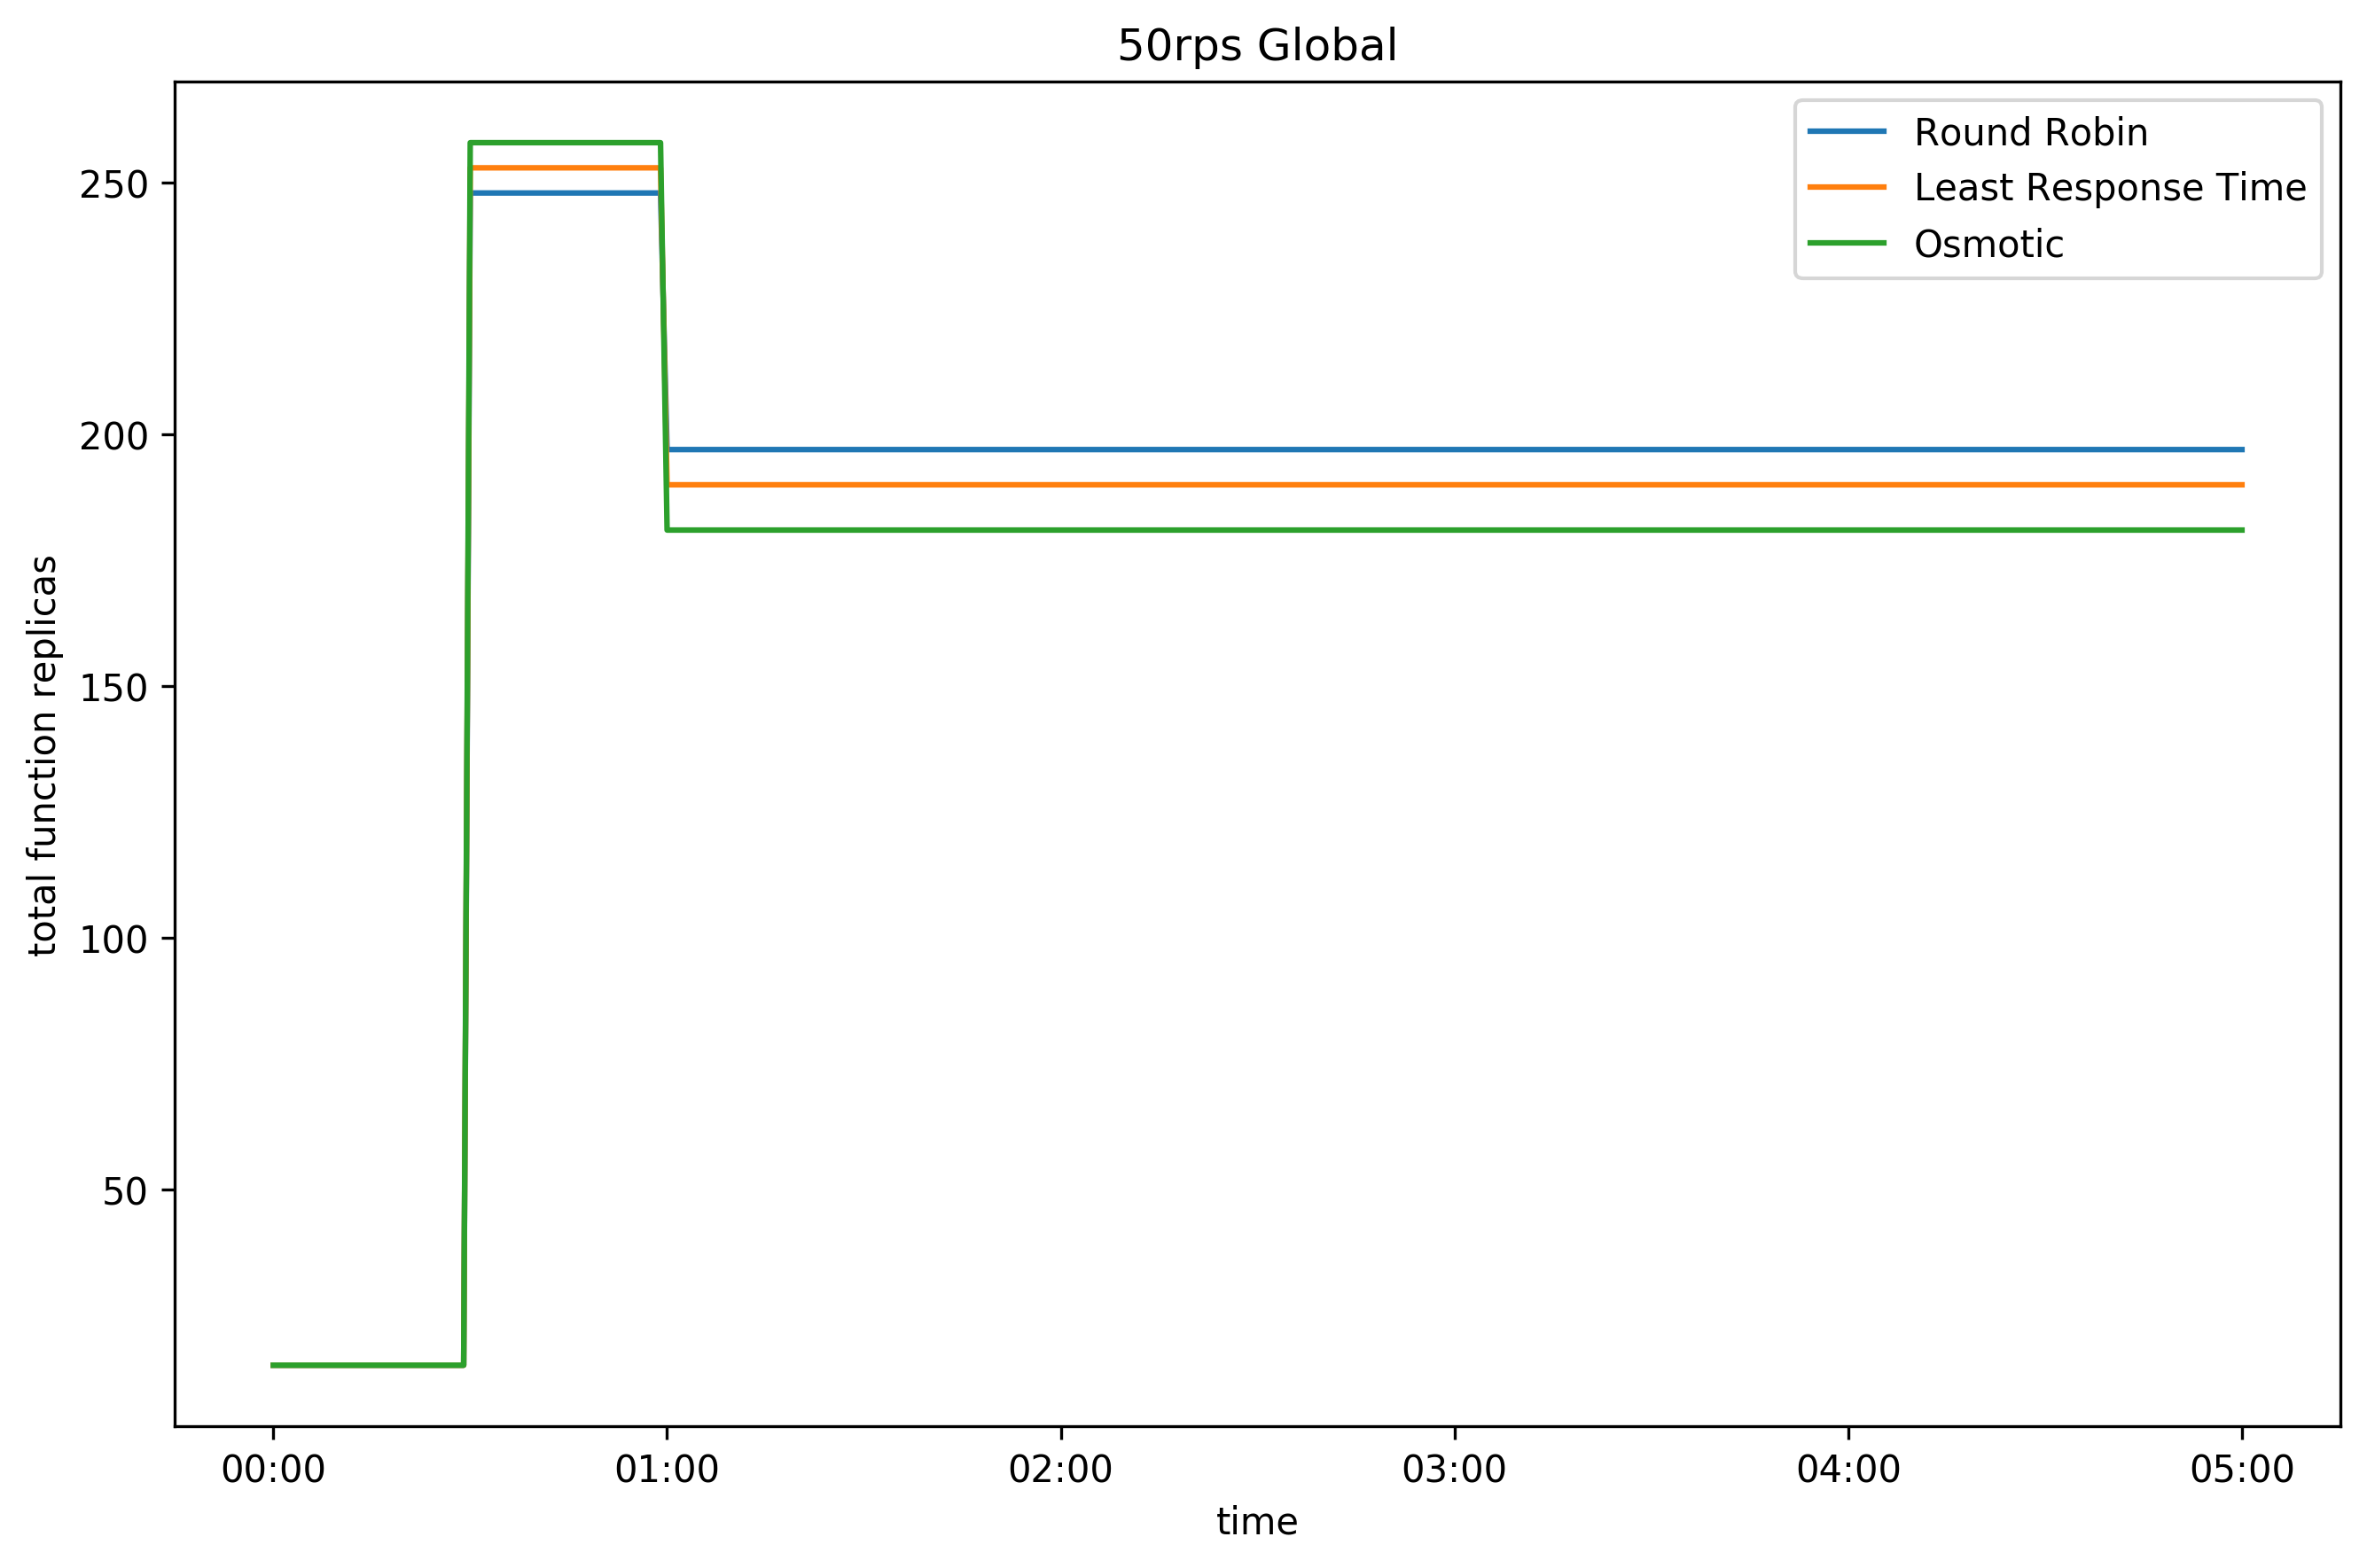
\includegraphics[width=12cm]{graphics/graphs/osmotic_base_function_scale_by_lb.png}
    \caption{Total scale of all functions for each load balancer scaling/schedulilng method}
    \label{fig:osmotic_fx_scale_by_scaling}
\end{figure}

Table \ref{tab:osmotic_base} shows the results of the experiment.
In terms of mean \gls{trt} performance the results of our proposed osmotic scaling and scheduling method are similar to those of the fixed scaling LRT reference setup, albeit between 1\% and 45\% worse with most scenarios only between 2\% and 8\% worse.
Differences between least response time static, and osmotic scaling are less pronounced in the median and 90th percentile \glspl{trt} as can also be seen in Table \ref{tab:osmotic_base}.
The statically scaled round robin load balancing is, as one would expect, significantly worse.
It does, however, give a good impression of the performance improvements possible based on our approach in a more complex and realistic deployment scenario than the initial evaluation.

We can also observe that in the city scenario the osmotic scaling and scheduling ends up deploying the more load balancer instances than the static scaling, but that for the nation- and globally-distributed network topology scenarios this patterns is reversed. There the osmotic scaler deploys only about a third of the replicas of the static scaling.

A similar pattern can be seen with regard to function scaling.
The osmotic scaling leads to between 1\% and 6\% fewer function replicas being deployed. Figure \ref{fig:osmotic_fx_scale_by_scaling} shows how the timing and frequency of scaling decisions are not different between the scaling methods, but osmotic scaling results in slightly fewer function replicas. 
\subsection{Optimization Aggressiveness with Osmotic Scaling}
We already learned from the experiment about load balancer scale that there is a tendency for a higher scale of load balancers to ultimately result in better performance.
With this experiment we want to test the interplay of this phenomenon with the osmotic load balancing and scaling we propose. With our osmotic approach we can set the scale-up threshold to more or less arbitrary values to influence how quickly or slowly the system scales up the number of load balancers, and how many load balancers will thus ultimately end up being deployed.

\subsubsection{Setup}
To test the performance we simulate a number of different configuration scenarios. For the rest of the system environment we choose to reuse the globally distributed topology from previous experiments with a request rate of 75\gls{rps} being simulated over the course of 2000 seconds.

For the parameters of the osmotic scaling and scheduling we run experiments for a range of scale-up thresholds ranging from 0.02 to 0.1.
The scale down threshold is always set to 0.2, which is relatively high, because we explicitly want to test how the scale-up threshold can be used to determine how many load balancers the system will deploy to optimize response times.

\subsubsection{Results}

\begin{table}[]
\begin{tabular}{lrrrrr}
\hline
\textbf{\begin{tabular}[c]{@{}l@{}}Upscaling\\ Pressure\\ Threshold\end{tabular}} & \textbf{\begin{tabular}[c]{@{}r@{}}LB\\ Replicas\end{tabular}} & \textbf{\begin{tabular}[c]{@{}r@{}}Mean\\ TRT\end{tabular}} & \textbf{\begin{tabular}[c]{@{}r@{}}Mean\\ FET\end{tabular}} & \textbf{\begin{tabular}[c]{@{}r@{}}Mean\\ LB\_FX\end{tabular}} & \textbf{\begin{tabular}[c]{@{}r@{}}Mean\\ CL\_LB\end{tabular}} \\ \hline
0.1                                                                               & 4                                                              & 155.8ms                                                     & 29.1ms                                                      & 33.5ms                                                         & 92.7ms                                                         \\
0.09                                                                              & 4                                                              & 152.5ms                                                     & 29.7ms                                                      & 30.1ms                                                         & 92.2ms                                                         \\
0.08                                                                              & 6                                                              & 152.1ms                                                     & 29.5ms                                                      & 30.0ms                                                         & 92.2ms                                                         \\
0.07                                                                              & 5                                                              & 152.5ms                                                     & 29.3ms                                                      & 30.4ms                                                         & 92.4ms                                                         \\
0.06                                                                              & 5                                                              & 148.5ms                                                     & 29.6ms                                                      & 26.6ms                                                         & 91.6ms                                                         \\
0.05                                                                              & 5                                                              & 147.5ms                                                     & 29.9ms                                                      & 25.3ms                                                         & 91.3ms                                                         \\
0.04                                                                              & 5                                                              & 148.5ms                                                     & 29.8ms                                                      & 26.5ms                                                         & 91.5ms                                                         \\
0.03                                                                              & 7                                                              & 136.8ms                                                     & 26.4ms                                                      & 19.6ms                                                         & 91.2ms                                                         \\
0.02                                                                              & 20                                                             & 139.0ms                                                     & 24.8ms                                                      & 25.3ms                                                         & 90.2ms                                                         \\ \hline
\end{tabular}
\caption{Response time performance metrics for different upscaling pressure thresholds}
\label{tab:osmotic_scaling_aggressiveness}
\end{table}





\begin{figure}
    \centering
    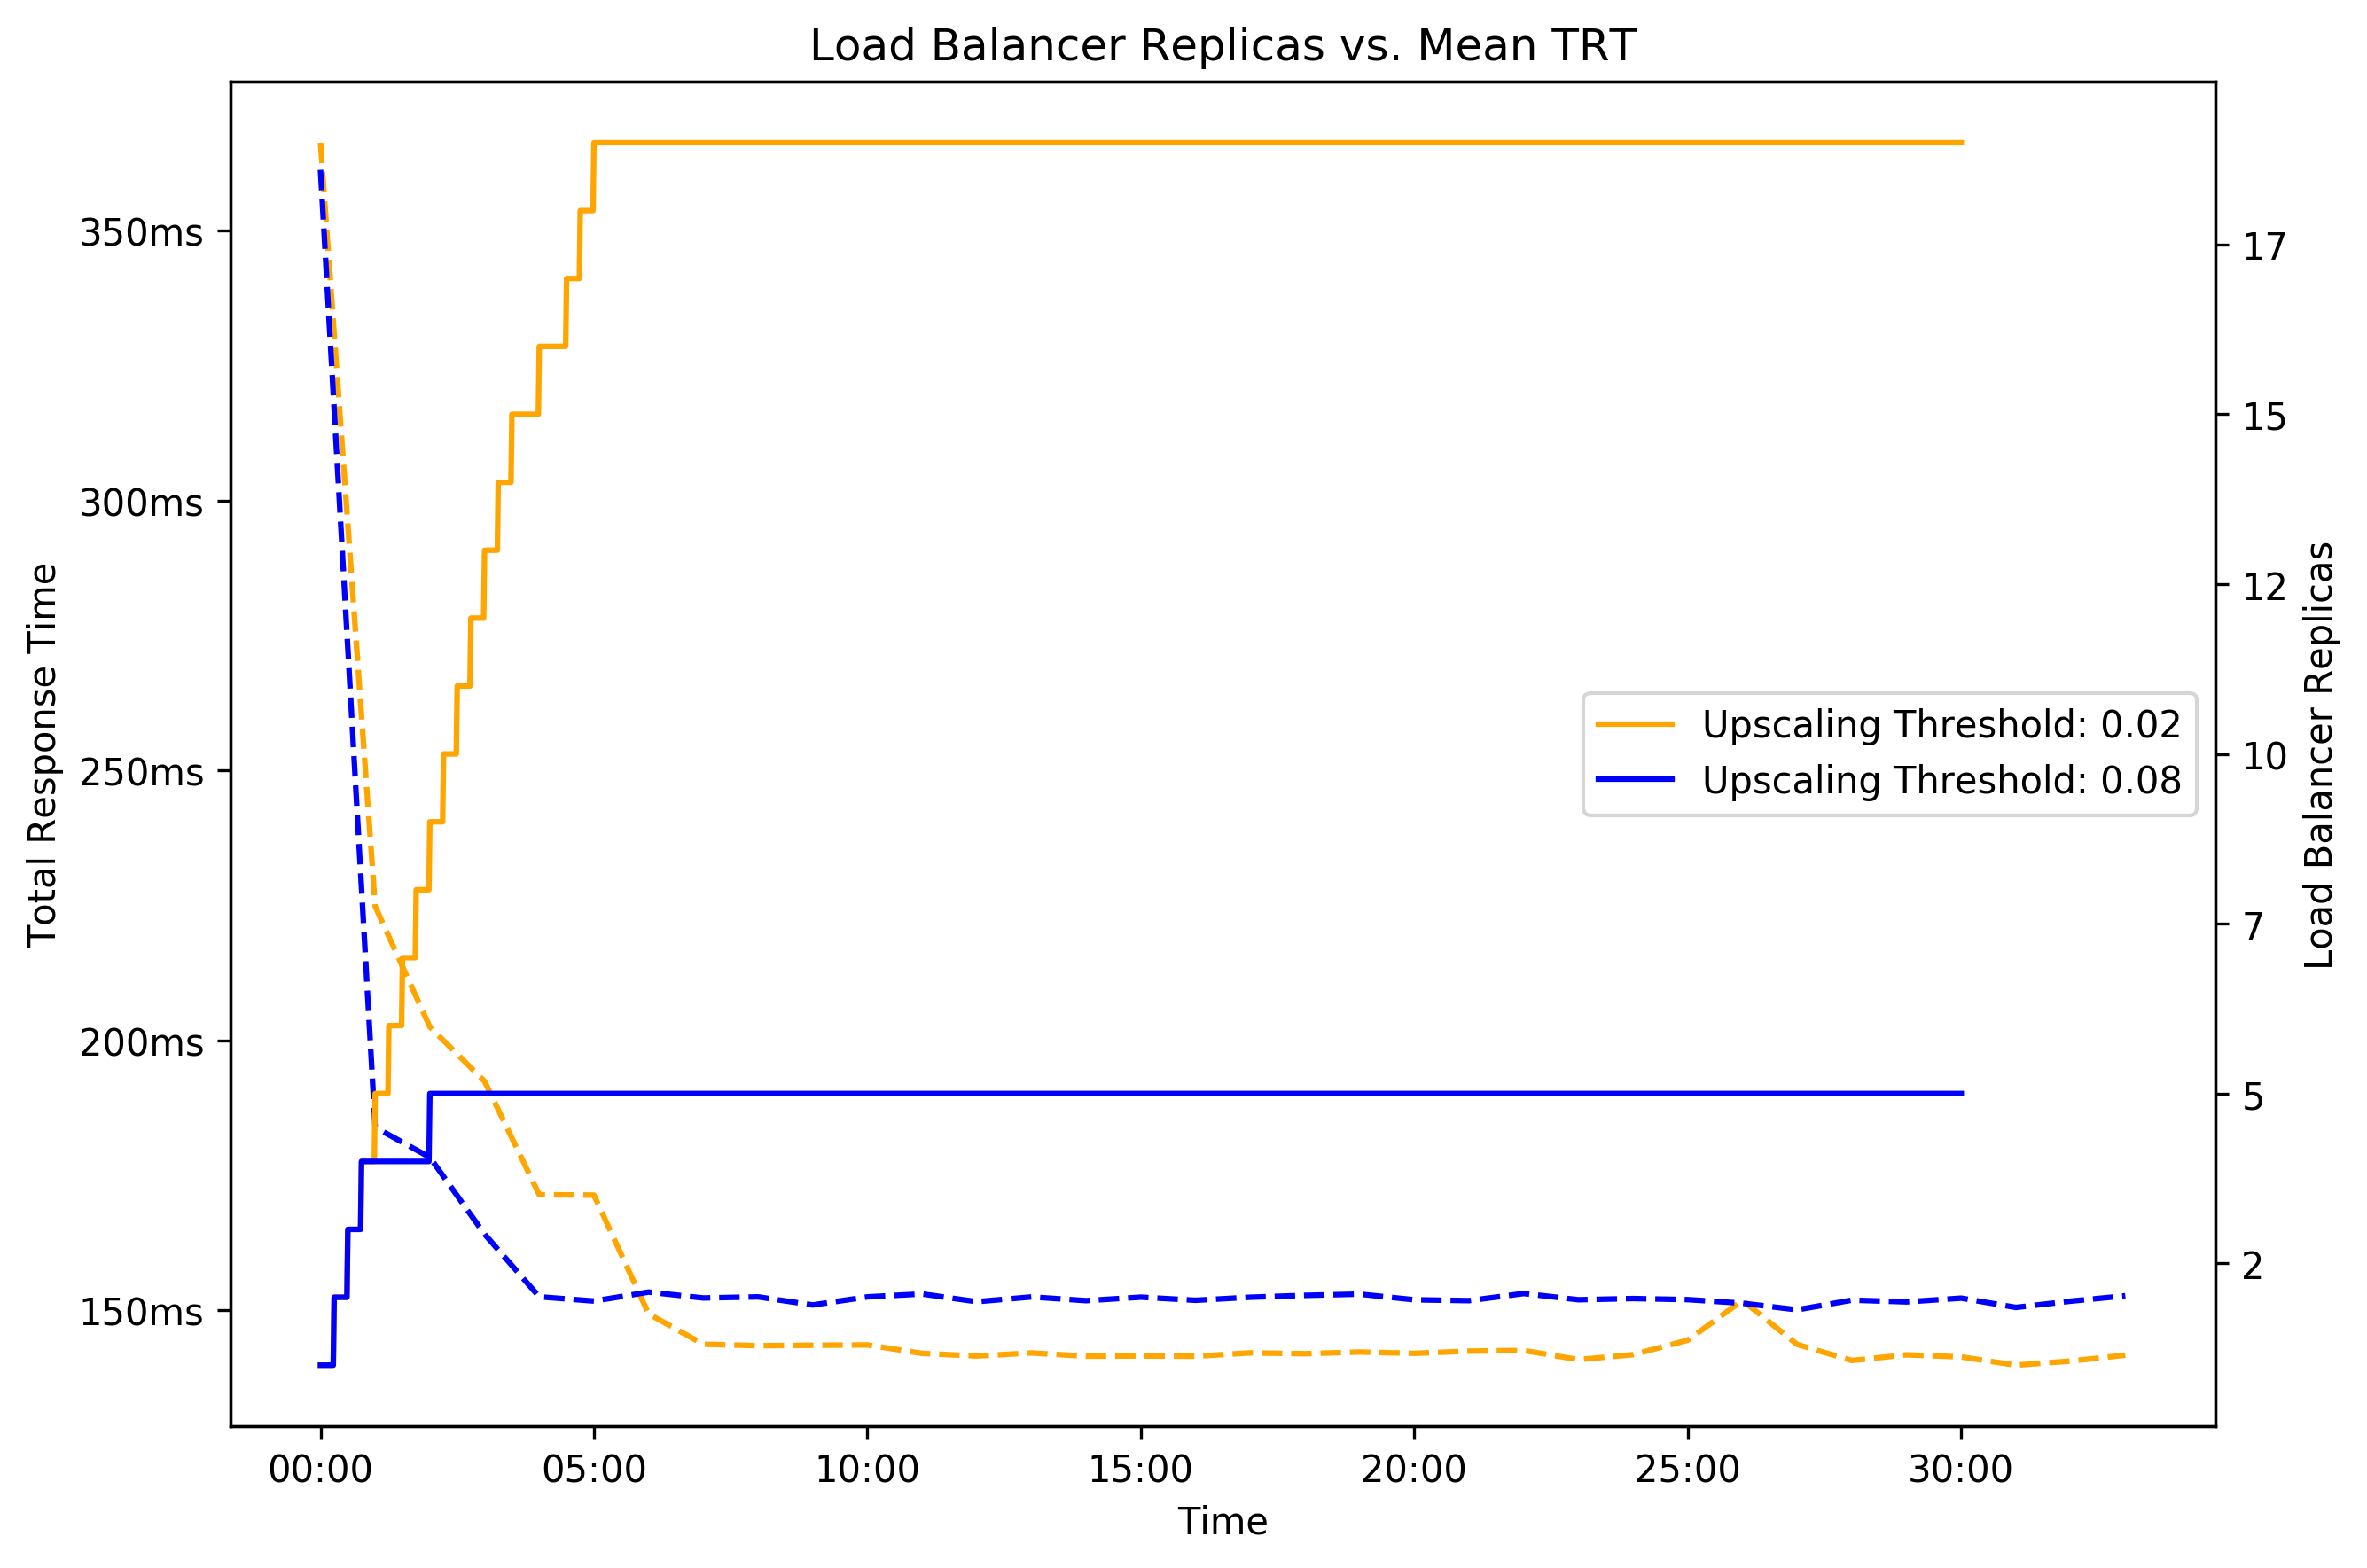
\includegraphics[width=12cm]{graphics/graphs/osmotic_optim_thres_vs_trt_corrected.png}
    \caption{\gls{trt} compared to current load balancer scale for two different osmotic scaling parametrizations}
    \label{fig:osmotic_trt_vs_replica_scale}
\end{figure}

The results show two clear trends.
First that will lower upscaling pressure thresholds more load balancer replicas are being deployed by the osmotic scaling component, and second that the mean response time improves with higher number of load balancer replicas.
As Table \ref{tab:osmotic_scaling_aggressiveness} shows, there is a diminishing return with higher numbers of load balancers, at least in the topology scenario tested.
The results also show that while higher numbers of load balancers provide better performance once the load balancers have gathered enough information about available replicas, this process is faster the fewer load balancers there are, thus giving better performance early on.
The behaviour can be observed easily in the graph in Figure \ref{fig:osmotic_trt_vs_replica_scale}.
\subsection{Osmotic Scheduling in Dynamic Systems}
% 3+ pages (complicated setup, no?)
In this last experiment we test the behaviour of our osmotic scaling and scheduling method in a dynamic system.
Since dynamic changes of the system make-up are a core part of edge computing, and our approach is explicitly constructed with these dynamic factors in mind, we believe it is important to test the efficacy of our approach in such a scenario.
Because a lot of components have already been analyzed in-depth, and results are most clear when only one factor is tested at any given time, we choose to use the request origin as the dynamic  system component.
With the experiment we test how our proposed approach handles requests originating from different regions of the overall system over time.
\subsubsection{Setup}
For this experiment we once again use the globally distributed scenario as our network topology, and apply a constant request rate of 25\gls{rps}.
Each of the three cities present in the topology additionally has a probability function associated with it, which determines the chance of a request originating from that city.
These probability functions for the cities are set up in such a way that most of the requests originate from only one of the cities for a given time period.
After some time the active city changes and the requests gradually start to come from another city.
The periods and changes are set up in such a way that over the course of the 2000 second long simulation each of the cities is the main originator of requests at one point.

\subsubsection{Results}

\begin{figure}
    \centering
    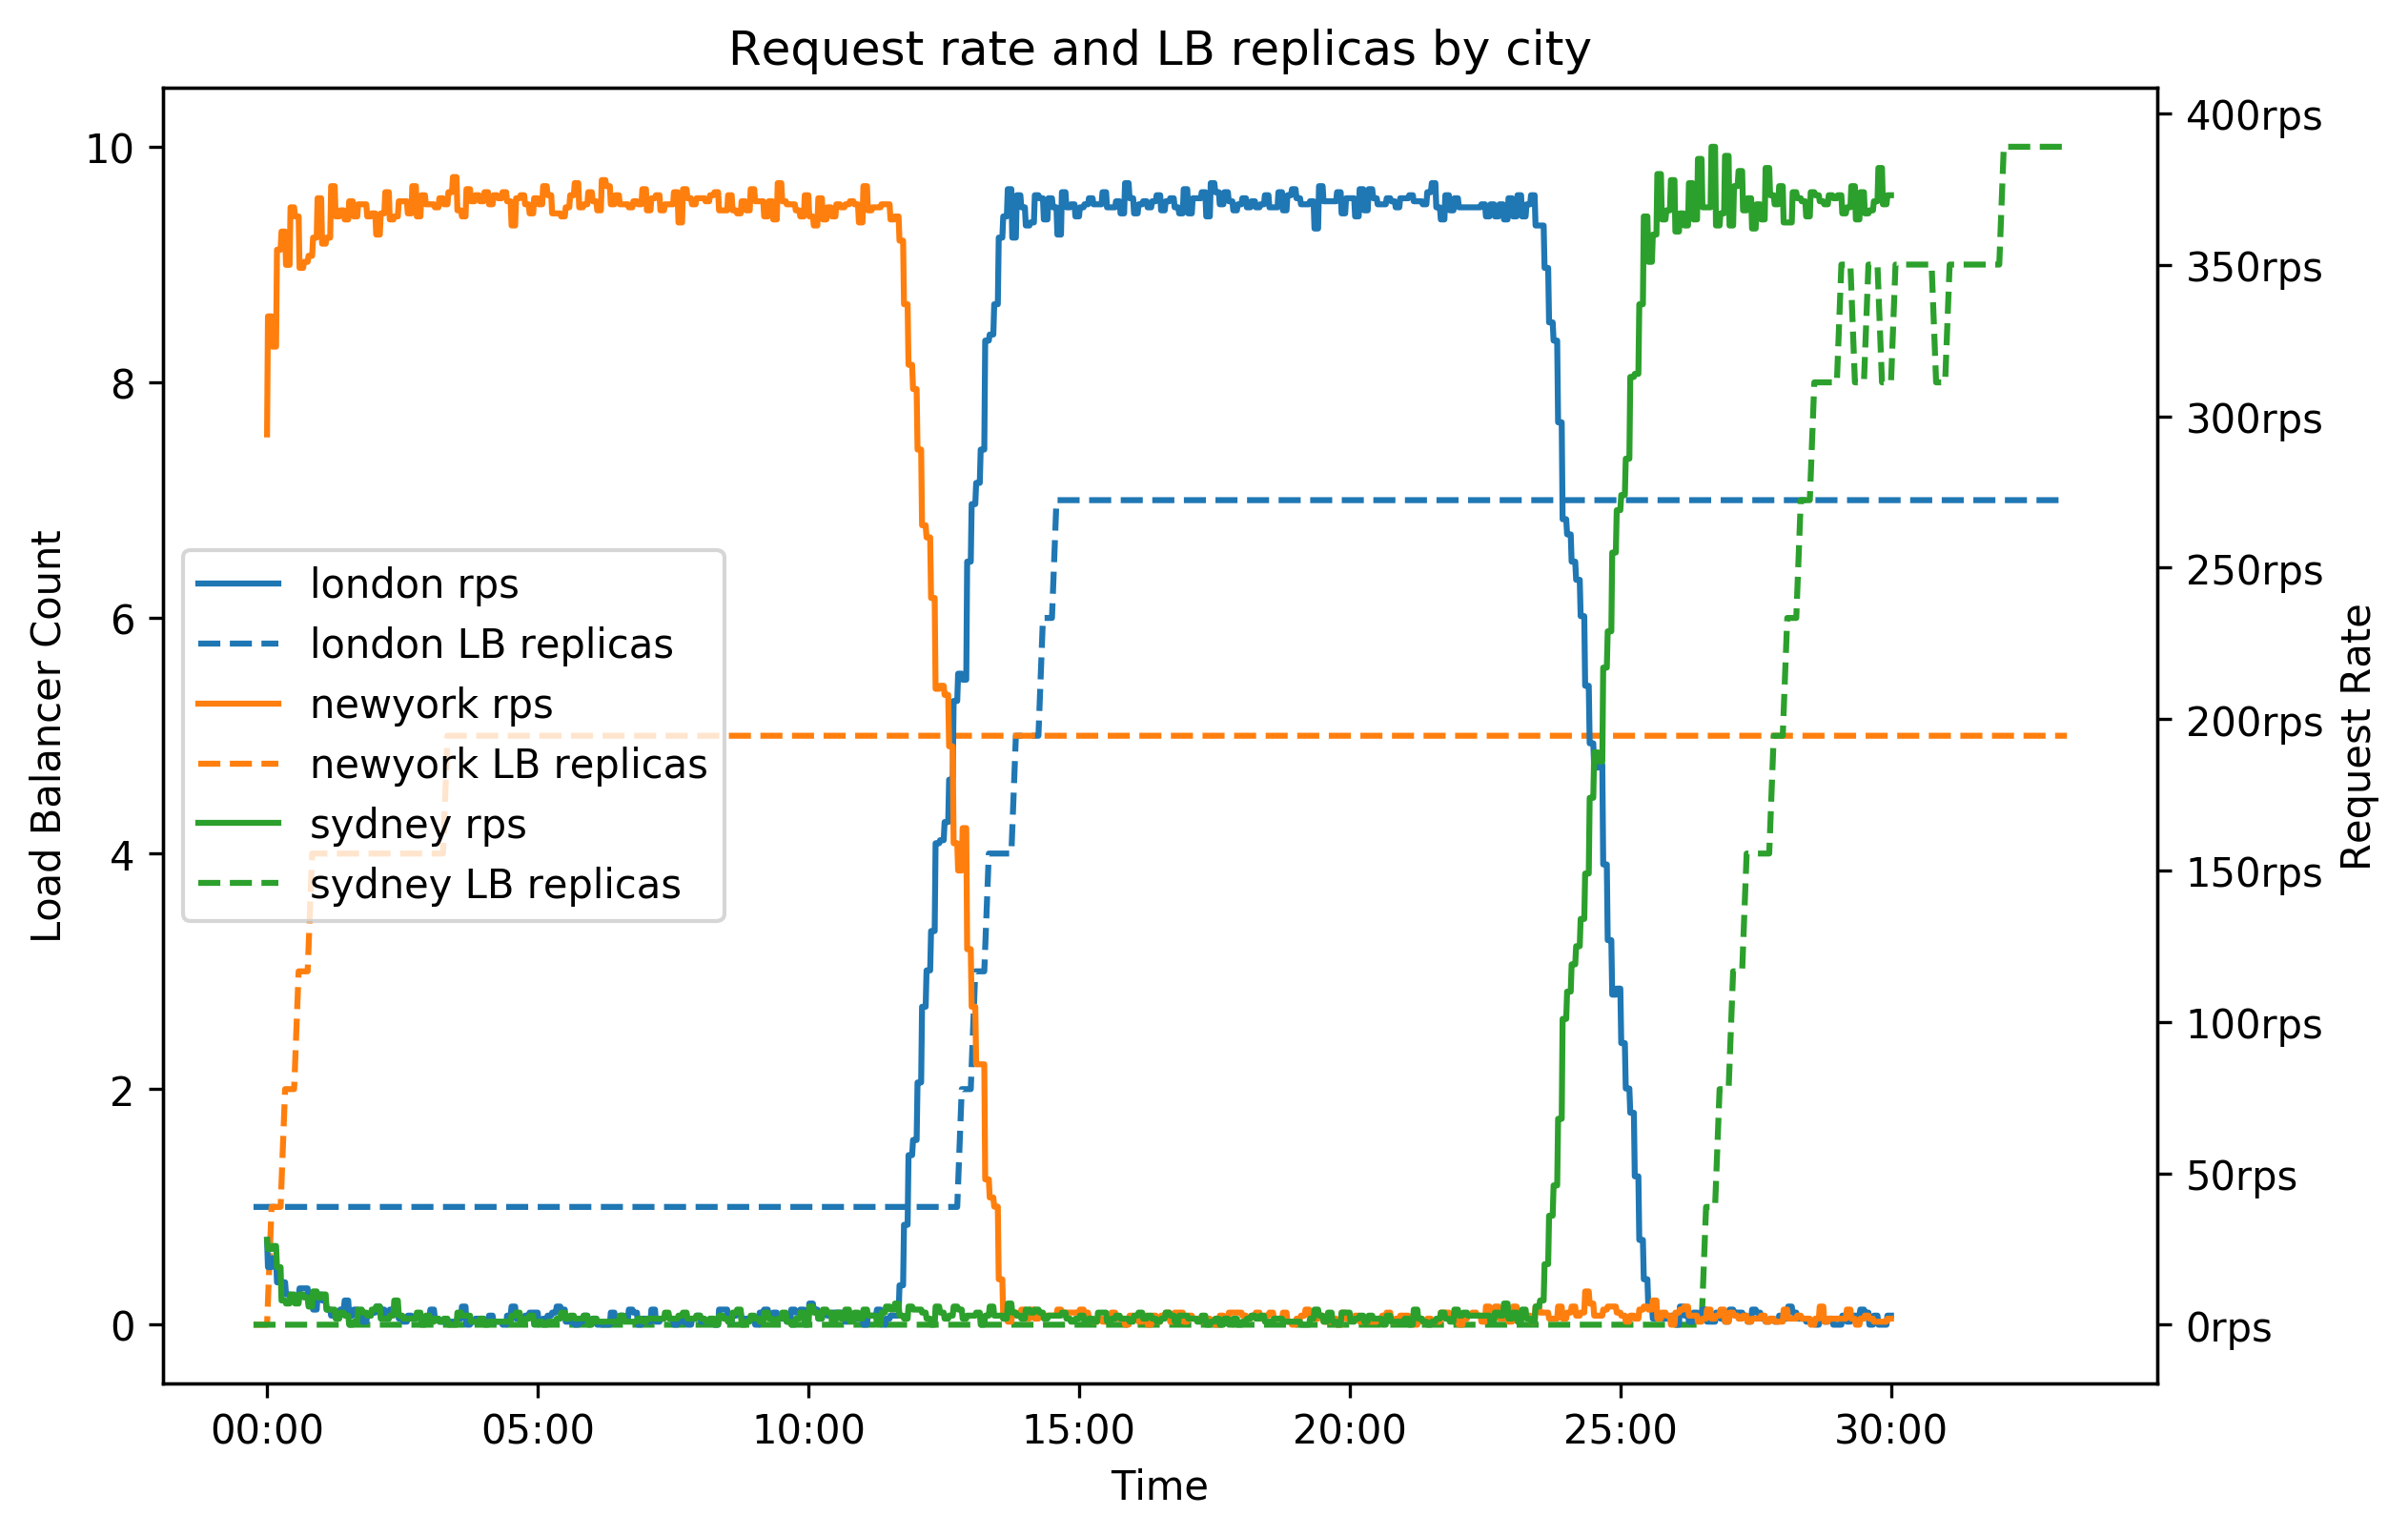
\includegraphics[width=14cm]{graphics/graphs/osmotic_dynamic_region_rps_lb_relicas_corrected.png}
    \caption{Load balancer replica count per city over changing request origins}
    \label{fig:osmotic_dynamic_lb_replicas}
\end{figure}

\begin{figure}
    \centering
    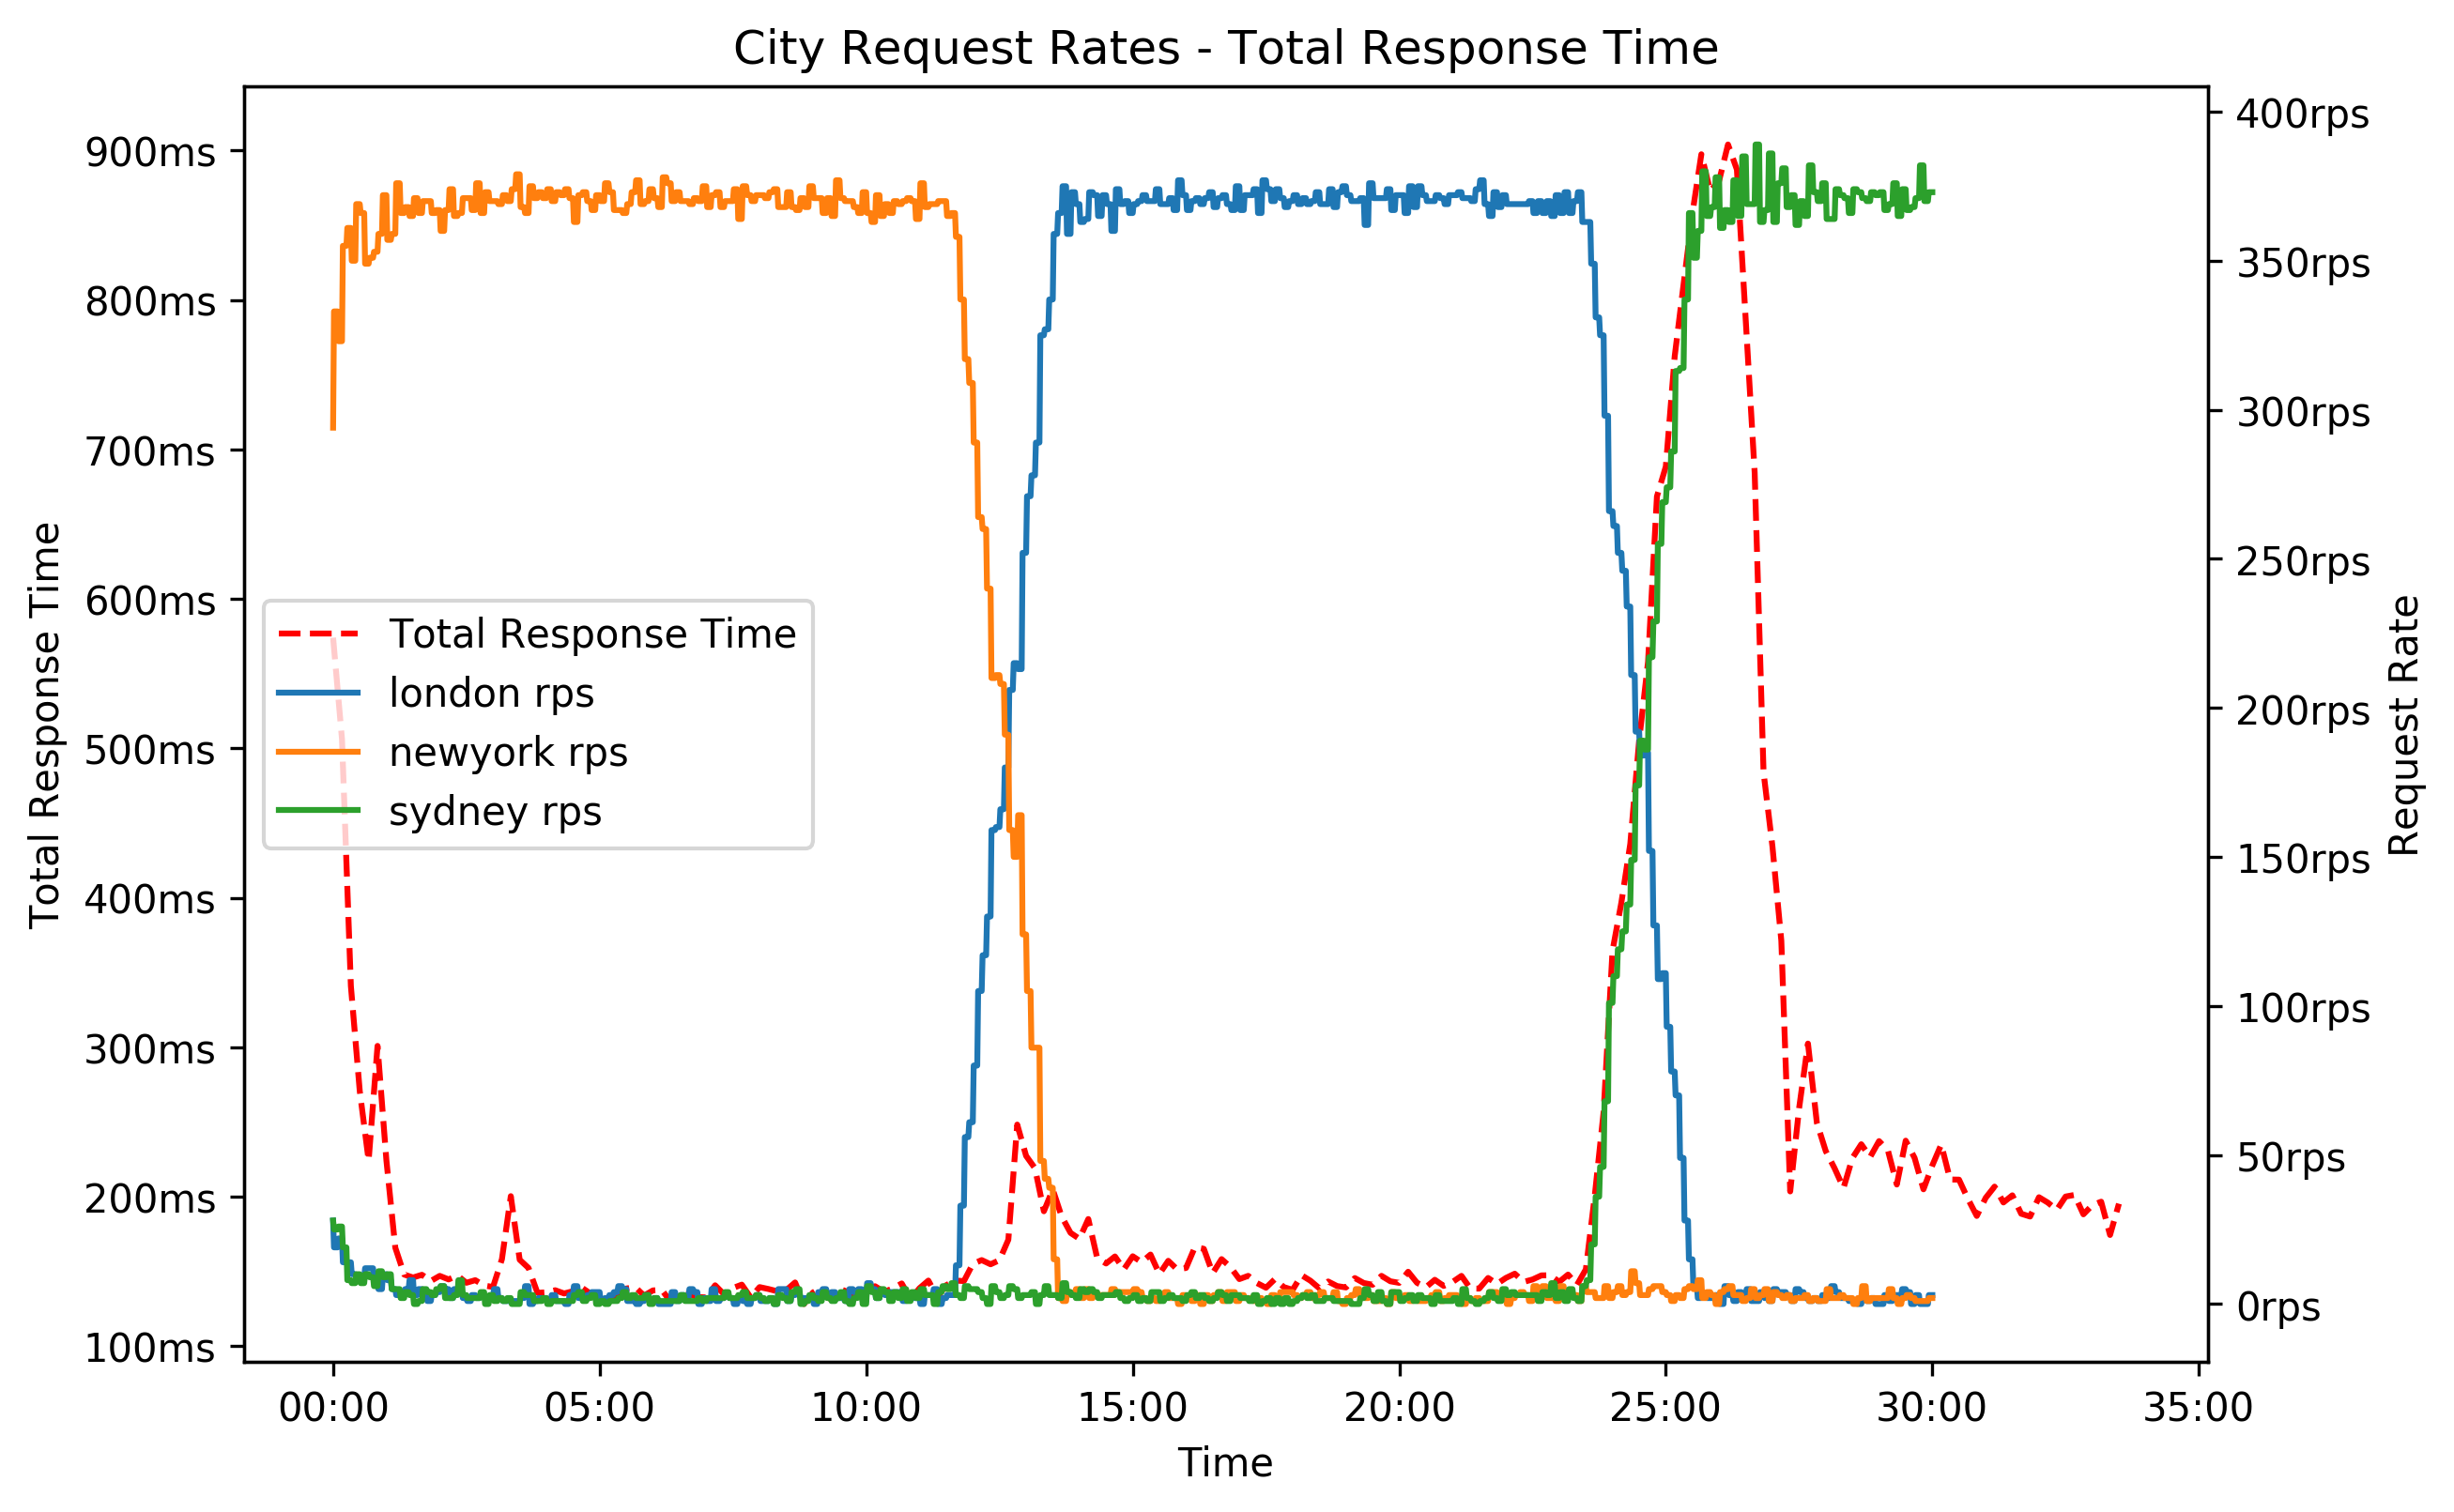
\includegraphics[width=14cm]{graphics/graphs/osmotic_dynamc_region_rps_trt_corrected.png}
    \caption{Total response time over changing request origins}
    \label{fig:osmotic_dynamic_trt}
\end{figure}

\begin{figure}
    \centering
    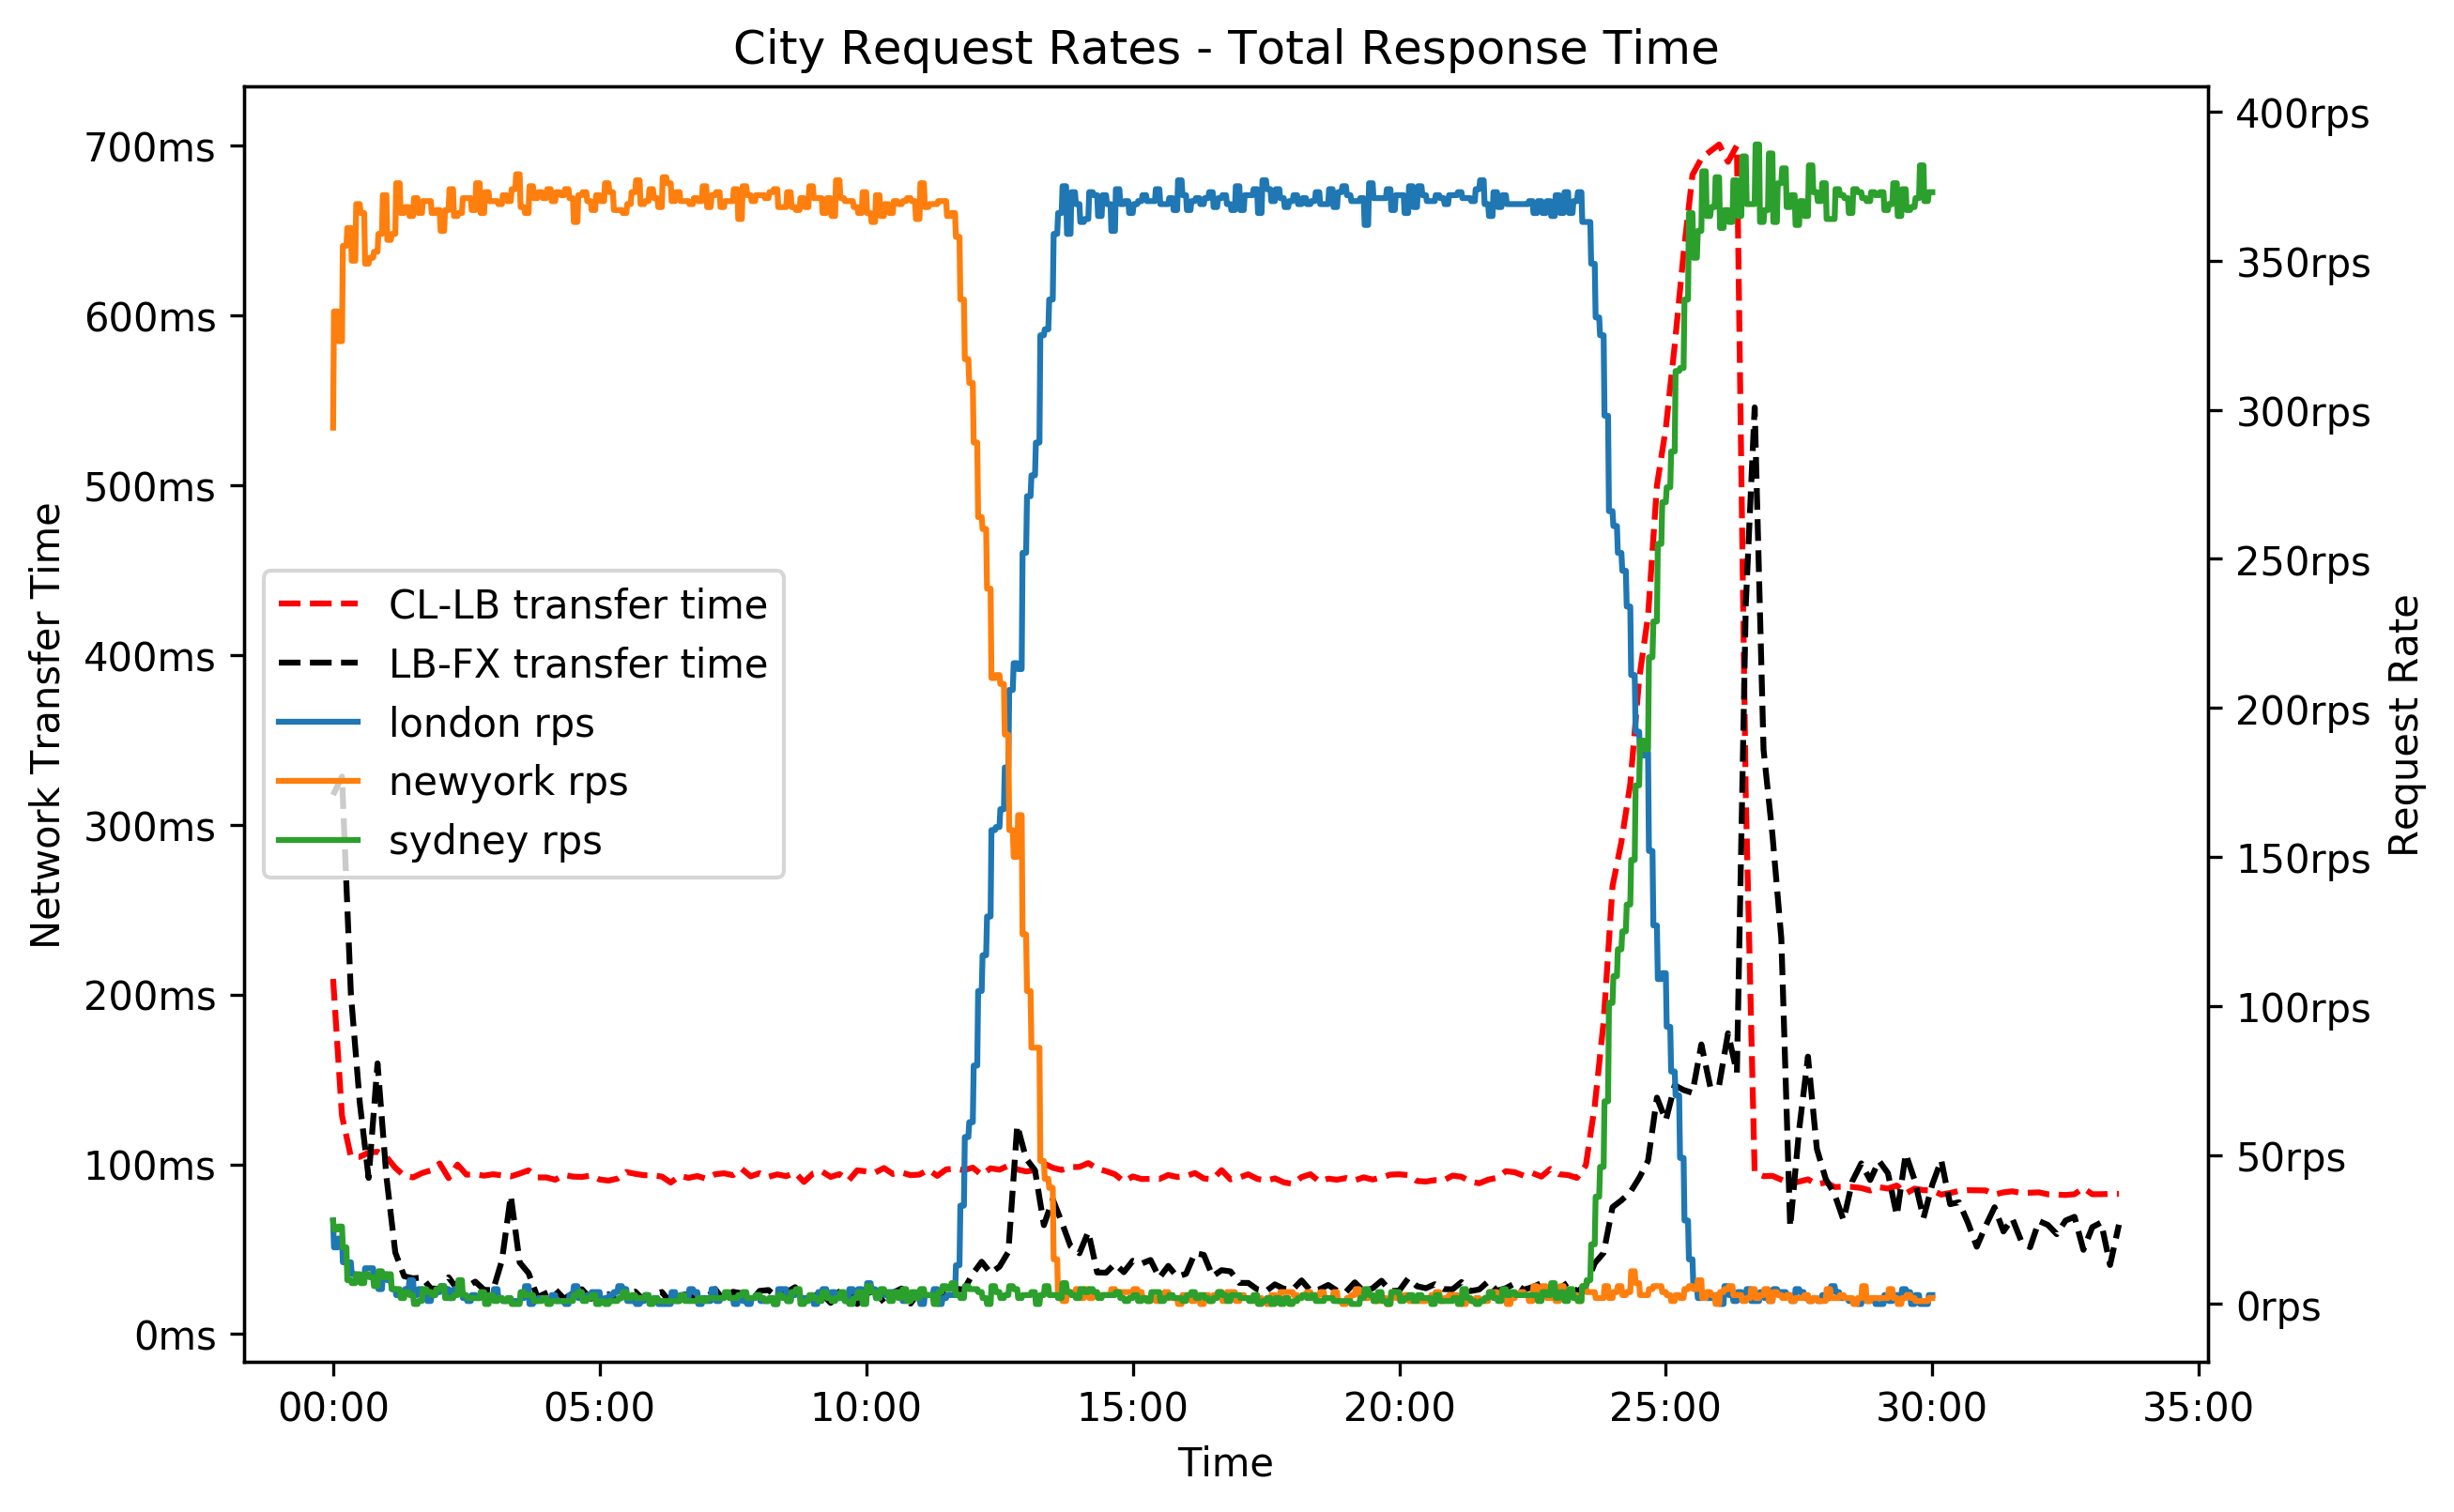
\includegraphics[width=14cm]{graphics/graphs/osmotic_dynamic_region_tx_times_corrected.png}
    \caption{Client to load balancer, and load balancer to function transfer times over changing request origins}
    \label{fig:osmotic_dynamic_tx}
\end{figure}

First of all, the results show that the osmotic scaling and scheduling component does indeed take the request origin into account when deciding on the number and location of new load balancer replicas.
Figure \ref{fig:osmotic_dynamic_lb_replicas} shows this in action.
While originally load balancers are only spawned in one city, because all requests originate from it, once requests start coming from another city, another load balancer instance is deployed in that city, as can be seen around timestamps 00:12 and 00:25 in Figure \ref{fig:osmotic_dynamic_lb_replicas}.

The effect this has on the system at large can also be observed easily, as Figure \ref{fig:osmotic_dynamic_trt} shows.
Here we can see that while the total response time of the system spikes once requests start to originate from another city, it starts to stabilize and come down to previous levels again once load balancers are present in the new city.
Please note that the \gls{trt} values shown in Figure \ref{fig:osmotic_dynamic_trt} are a moving average over a 10 second window, since this removes noise from the plot, making it more readable.
Likewise the request rate per city in Figures \ref{fig:osmotic_dynamic_lb_replicas}, \ref{fig:osmotic_dynamic_trt}, and \ref{fig:osmotic_dynamic_tx} is a moving average over a 5 second window, and displays the request rate for all functions deployed in the system.

Just like with the \gls{trt}, Figure \ref{fig:osmotic_dynamic_tx} shows that the request transfer time between client and load balancer, as well as between load balancer and function replica also spike when traffic originates from a different city.
There too, though we see that it returns to previous levels once load balancer replicas become available near the request origin.
